\documentclass[11pt]{report}

%Margin Setting
\usepackage[left=1.4in, right=1.4in, top=0.8in, bottom=1.0in,includefoot]{geometry}
\usepackage{pgfplots}

% Fonts
\usepackage[T1]{fontenc}
\usepackage[utf8]{inputenc}

% \usepackage{kpfonts}

% Titles
\usepackage{titlesec, blindtext, color}
\usepackage{fmtcount}
\newcommand{\hsp}{\hspace{20pt}}
\titleformat{\chapter}[display]
  {\centering\normalfont\Large\bfseries}
  {\MakeUppercase {\chaptertitlename\ \NUMBERstring{chapter}}}
  {0pt}
  {\MakeUppercase}
% \titleformat{\chapter}[hang]{\huge\bfseries}{\thechapter \hsp }{0pt}{\huge\bfseries}
\titlespacing*{\chapter}{0pt}{-20pt}{30pt}

\titleformat*{\section}{\Large\bfseries}
\titleformat*{\subsection}{\large\bfseries}
\titleformat{\subsubsection}[hang]
	{\normalfont\fontsize{11}{12}\bfseries}
	{}
	{0em}
	{}
	
% List of Tables and figures
\usepackage{tocloft}
\makeatletter
\def\ext@figure{lot}
\def\ext@lstlisting{lot}
\makeatother
\renewcommand{\cftfigpresnum}{Figure~}
\renewcommand{\cftfigaftersnum}{:}
\setlength{\cftfignumwidth}{5.5em}
\renewcommand{\cfttabpresnum}{Table~}
\renewcommand{\cfttabaftersnum}{:}
\setlength{\cfttabnumwidth}{5.5em}

\renewcommand*\listtablename{List of Figures and Tables}

\usepackage{float}
\usepackage{placeins}
\usepackage{subfig}

% Paragraphs and Line Spacing
\linespread{1.5} 

% Table of Contents
\renewcommand{\contentsname}{\hfill\normalfont\Large\bfseries\MakeUppercase{Table of Contents}}
\renewcommand{\listtablename}{\hfill\normalfont\Large\bfseries\MakeUppercase{List of Figures and Tables}}
\renewcommand{\cftaftertoctitle}{\hfill}
\renewcommand{\cftafterlottitle}{\hfill}

\setlength{\cftbeforetoctitleskip}{-20pt}
\setlength{\cftaftertoctitleskip}{30pt}

\setlength{\cftbeforelottitleskip}{-20pt}
\setlength{\cftafterlottitleskip}{30pt}

\setlength\cftparskip{-2pt}
\setlength\cftbeforechapskip{0pt}


%Page Number and Header+Footer
\usepackage{fancyhdr}
\pagestyle{fancy}
\fancyhead{}
\fancyfoot[C]{\thepage}
\renewcommand{\headrulewidth}{0pt}
\renewcommand{\footrulewidth}{0pt}
\usepackage{textcomp}
\pgfplotsset{compat=1.16}

% Lists
\usepackage{enumitem}

%Chapter
\usepackage[T1]{fontenc}
\usepackage{titlesec, blindtext, color}

%Tables
\usepackage{booktabs}% http://ctan.org/pkg/booktabs
\newcommand{\tabitem}{~~\llap{\textbullet}~~}
\usepackage{multirow}
\usepackage{caption} 
\usepackage{tabularx}
\usepackage{longtable, tabu}
\usepackage{ltablex}
\captionsetup[table]{skip=10pt}

%Maths
\usepackage{amsmath}
\usepackage{amssymb}
\usepackage{amsfonts}
\usepackage{amsthm}
\newcommand*\VF[1]{\mathbf{#1}}
\newcommand*\dif{\mathop{}\!\mathrm{d}}
\newtheorem{theorem}{Theorem}[section]
\newtheorem{corollary}{Corollary}[theorem]
\newtheorem{lemma}[theorem]{Lemma}

%Code Hilighting
\usepackage{listings}
\usepackage{xcolor}

\definecolor{codegreen}{rgb}{0,0.6,0}
\definecolor{codegray}{rgb}{0.5,0.5,0.5}
\definecolor{codeorange}{rgb}{255,127,80}
\definecolor{backcolour}{rgb}{255,255,255}

\lstdefinelanguage{json}
{
    morestring=[b]",
    morestring=[d]'
}

\lstdefinestyle{mystyle}{
    backgroundcolor=\color{backcolour},   
    commentstyle=\color{codegreen},
    keywordstyle=\color{blue},
    numberstyle=\tiny\color{codegray},
    stringstyle=\color{orange},
    basicstyle=\ttfamily\footnotesize,
    breakatwhitespace=false,         
    breaklines=true,                 
    captionpos=b,                    
    keepspaces=true,                 
    numbers=left,                    
    numbersep=5pt,                  
    showspaces=false,                
    showstringspaces=false,
    showtabs=false,                  
    tabsize=2
}

\lstset{style=mystyle}


%Photos
\usepackage{graphicx}
\usepackage{float}

%Links
\usepackage{hyperref}
\hypersetup{
    colorlinks=true,
    linkcolor=black,
    filecolor=magenta,      
    urlcolor=blue,
    citecolor = black,
}

%Date
\usepackage[nodayofweek,level]{datetime}
\newdateformat{monthyeardate}{%
  \monthname[\THEMONTH], \THEYEAR}
  
%Bibliography
\renewcommand\bibname{References}

% Directories
\usepackage{dirtree}
\input dirtree
\usepackage{etoc}

  
\begin{document}
%--------------------------------------------------------
% Front Matter
%--------------------------------------------------------
\begin{titlepage}
	\begin{center}
	
\includegraphics[scale = 0.5]{Images/kings.jpg}\\
	[1cm]
	\hrule 
	\vspace{0.5cm}
	\huge{\bfseries Machine Learning and Virtualisation Techniques Applied to Cyber Intrusion Detection}\\
	\vspace*{\fill}
	\large{Kenan-Ali Jasim}\\
	\large{BEng Electronic and Information Engineering }\\
    \vspace*{\fill}
	\large{\textbf{Student ID}: 1735764}\\
	\large{\textbf{Supervisor}: Prof. Mischa Dohler}\\
	\textsc{\large 	King's College London \\ \today\\}
	\end{center}
\end{titlepage}
\pagenumbering{roman}
\chapter*{abstract}
\addcontentsline{toc}{chapter}{\numberline{}Abstract} 
An Intrusion Detection System (IDS) conventionally uses signature-based detection. This approach works by identifying specific patterns associated with an attack, such as byte sequences in network traffic to a database of known attacks. This approach has two major limitations. It requires extensive, expert lead configuration and cannot detect zero-day (novel) attacks.

A new approach to IDS involves anomaly-based detection, leveraging recent advancements on Data Mining and Machine Learning technologies to profile normal behaviour and then detect anomalies/indicators of compromise. Typically, this is implemented using algorithms such as K-Nearest Neighbour or Fuzzy logic). This technology has been successfully implemented at production level within financial fraud detection, but is still emerging within cyber-security. This approach requires a large amount of data, however, which is lacking in the cybersecurity community.

The goal of the project is to implement an automated visualised network that can generate a large amount of data from a wide range of configurable threats. This data will then train a decision tree model to create an Intrusion Detection Model. The technology will mainly rely on decision trees for their 'explainability'. Demonstrated success in this under-researched area would be an important step in cybersecurity systems.
%Originality Avowal
	\chapter*{Originality Avowal}
	\addcontentsline{toc}{chapter}{\numberline{}Originality Avowal} 
  	\begin{center}
                        \begin{flushleft}
			I verify that I am the sole author of this report, except where explicitly stated to the contrary.
			I grant the right to King's College London to make paper and electronic copies of the submitted work for purposes of marking, plagiarism detection and archival, and to upload a copy of the work to Turnitin or another trusted plagiarism detection service. I confirm this report does not exceed 25,000 words.\\
			\end{flushleft}
  		\begin{flushright}
        		      \normalsize{Kenan-Ali Jasim}\\*
		      \normalsize{\today}\\*
		      %\normalsize{Word count: \@wordCount}
  		\end{flushright}
  	\end{center}
\chapter*{Acknowledgements}
\addcontentsline{toc}{chapter}{\numberline{}Acknowledgements} 
I would like to thank my project supivisor Prof. Mischa Dohler for his support throughout the project. I would also like to thank my parents, my family and my friends for their unwavering support and encouragement throughout the project.
\newpage
\vspace*{\fill}
\begin{center}
\textit{For my late uncle Ali Fahs, may he rest in peace.}
\end{center}
\vspace*{\fill}
\newpage
%--------------------------------------------------------
% Table Of Contents
%--------------------------------------------------------
\tableofcontents
%--------------------------------------------------------
% List of figures and tables
%--------------------------------------------------------
\newpage
\listoftables
\addcontentsline{toc}{chapter}{\numberline{}List of Figures and Tables}
%--------------------------------------------------------
% Main Section Configurations
%--------------------------------------------------------
\thispagestyle{empty}
\cleardoublepage
\pagenumbering{arabic}
\setcounter{page}{1}
%--------------------------------------------------------
% Introduction
%--------------------------------------------------------
\chapter{Introduction}
Security has always been of utmost concern since the Internet first became widely adopted in 1991 \cite{www}. Bob Thomas wrote the first ‘cybersecuirty’ threat in 1971 \cite{compvir}. The creeper worm was a virus designed to replicate itself on mainframe computers over the Internet. Since then, cybersecurity threats have become more sophisticated with governments waging wars over the Internet. Because of this, cybersecurity is now essential for safeguarding sensitive computer systems.

With the greater sophistication of network security threats, there needs to be more sophisticated tools at hand to counteract these threats. For a long time, a firewall was the only tool available for networks to remain secure, this however does not protect networks from threats entering open ports. 

Intrusion detection systems are pieces of software that run on a network and monitor activity. It focuses on two types of detection: Signature Based Detection and Anomaly Based Detection. Signature-based IDS refers to the detection of attacks by looking for specific patterns, such as byte sequences in network traffic. Threats which are unique can evade signature based detection.

The problem with this is that they are poor at identifying and classifying novel attacks, they can either tell you if you are being attacked and if the attack is known. “An attack need not be advanced or highly sophisticated to bypass most enterprise security defences. It just needs to be unique” \cite{avetco}.

A novel approach to IDS involves anomaly-based detection, leveraging recent advancements in Data Mining and Machine Learning to profile normal behaviour and then detect anomalies/indicators of compromise. Typically, this is implemented using algorithms such as k-nearest neighbour or fuzzy logic). 

A very large problem in the cybersecurity world is the unavailability of reliable and recent data, data mining techniques can only be as successful as the data which it has to work with. The best and most reliable data set, which is widely available, is the KDD99 data set \cite{kd99ds}, which is based on the DARP98 dataset and comprises processed and labelled network data. The issue with this dataset is that it is over 20 years old, making it a poor representation of the cybersecurity threats are of the highest concern now. 

For this reason, it is necessary to create a dataset to train the intrusion detection system. Attacking a target virtual machine generates network data that is collected and processed to form a dataset. Scripts are therefore needed to generate the virtual machines, attack the target machine, collect network data, and process said data.

The background will outline the project, its aims and motivations along with the research contributions made. The requirements and design will develop more specific requirements for the project to abide by and will design a system around it. The implementation chapter will detail the development of the project along with any issues experienced during implementation. The testing and evaluation sections will review the project and the conclusion section will suggest future work.

\section{Aims}
The project aims to develop a program able to automatically generate a virtualised network. A user should be able to write attack scripts to run on this virtualised network to generate attack data, which shall be used to build a personalised dataset. This personalised dataset will train a classifier which can be used in anomaly based intrusion detection.

The project will aim to package the program into a simple command based interface to be utilised by the user, they will not require high-level technical knowledge to generate a model. The system will utilise a pre-configured virtualised network for testing.

\section{Scope}
The cybersecurity and machine learning domains are broad fields which contain a sizeable amount of overlapping sections. To ensure that the project has the best chance of success the scope must be clearly defined, this ensures that the project will stay on track and not roam into areas which are not related. 

The project will focus on automating virtual networks and creating network data from this network. The project will not aim to develop novel attacks to utilise on this network. The sole aim of the project is to create the framework to be able to generate network data not to generate novel network attacks. Instead the utilisation of third-party software such as Metasploit will form the attack suite for this project.

The project will also test the generated dataset from a machine learning model. This will involve the utilisation of third-party machine learning algorithms and the generated dataset to create a model. The project will not aim to redevelop a machine learning module as the modules available are sufficient for the application.

\section{Own Research Contributions}

This project aim is to utilise virtual networks to provide an automated way of creating reliable datasets to train the model. This involves automating the creation of a virtual network, attacking the network with the required suite of threats and collecting the network data. Network administrators can generate sizeable amounts of data on a particular threat and use this data to strengthen their intrusion detection system. The project utilizes Packer, an open source tool created to automate the creation of virtual machine images. The virtualised network allows devices to communicate between each other. 

User written attack scripts are then run on the virtualised network through Packer, which allows the user to specify the attacks which they require in network data generation. The program also includes the ability to generate normal data as any anomaly based intrusion detection system must involve first modelling normal network behaviour.

Decision trees work by categorising data by moving down a tree and applying tests to the data to determine which branch is appropriate. Then the tree is split, recursively, until either there are no features to split by, no more data left or it can make a classification. It will return a class in all cases. The current state of both data sets and IDS in the cybersecurity world are miles behind the constant evolution of threats, creating a system where generated data for threats contribute to building a stronger intrusion detection system can allow a quicker response by cybersecurity tools. The sklearn library trains a decision tree classifier using the dataset generated from the virtualised network. Decision trees would be new for intrusion detection systems, with most signature detection implemented by scanning network data and matching signatures with data to classify threats, most anomaly detection implemented by K-nearest-neighbour or a neural network, and most of the research on decision trees lacking new data to model. 
%--------------------------------------------------------
% Background
%--------------------------------------------------------
%--------------------------------------------------------
%Literature Review
%--------------------------------------------------------
\chapter{Background and Literature Review}
This chapter will provide some background information into the concepts that are to be used in the project. The chapter examines virtualisation, intrusion detection systems, network attacks and classification techniques along with existing research in the field.

\section{Virtualisation}
Virtual machines allow the ability to simulate a standalone computer within a host PC. Hypervisors partition the resources of the computer to the virtual machines allowing it to run as a standalone PC. This project aims to utilise virtual machines to create virtual networks automatically and attack them to generate data.

\subsection{Virtualisation Software}
The choice is between the two most popular pieces of software, VMware and VirtualBox. Both are pieces of virtualisation software that would allow the running of virtual machines. They are very similar programs they both use a type 2 hypervisor and both support both hardware virtualisation\cite{vvv}. However, VirtualBox can run on more operating systems and supports software virtualisation while also being open source, which is both free and allows for future expansion \cite{vvv}. Therefore, VirtualBox will be used in the project.

\section{Intrusion Detection Systems}
Intrusion detection systems are pieces of software that monitor network data. They can be split into two main groups: Signature based intrusion detection systems and Anomaly-based intrusion detection systems. 

\subsection{Signature-based Intrusion Detection Systems}
Signature based IDS function by detecting previously seen and identified threatening patterns. A pattern may be a network packet or a sequence of commands that have been applied as part of some malware. A database of known patterns is stored, and the IDS compares these to the current pattern to see if there is a match. This gives great detection rates for threats which already exist within the database \cite{Khraisat2019} however detection of novel zero day threats is not possible as the signature does not exist within the database. 

\subsection{Anomaly-based Intrusion Detection Systems}
Anomaly-based IDS uses machine learning techniques to detect anomalous data. A model of normal activity is created through machine learning techniques, and any activity which does not align with this is considered an anomaly \cite{Khraisat2019}. This allows for zero-day threats to be detected as there is no requirement for the pattern to be in some database. Anomaly-based methods tend to have a high rate of false positives, as any action not aligned with the normal model is considered anomalous. They also cannot give specific information about the threat, often just raising an alarm.

\section{Machine Learning}
\subsection{Classification}
Classification is defined as learning a function that, given a set of attributes returns the class which this data best fits into \cite{I2DM}.
\begin{figure}[H]
\centering
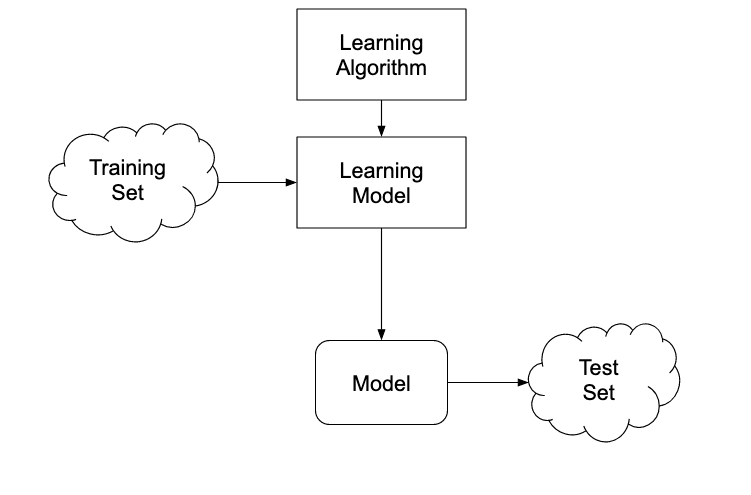
\includegraphics[scale = 0.3]{Images/classification.png}
 \caption{Generalised approach to classification problem}
 \label{fig:class}
\end{figure}
Most classification models follow a similar approach, which is detailed in Figure \ref{fig:class}. A model is learned by applying data in a training set to a learning algorithm, once the model is learned its accuracy is measured by applying it to some test data. If a row in the test data passes the classification threshold for a certain class, it is considered part of that class. The labels for each row of the test data is known, and the model is evaluated based on the accuracy of its prediction \cite{I2DM}.

\subsubsection{Evaluation}
Evaluation is generally based on the number of correct and incorrect labels that the model assigns to the test data. 
\begin{equation}\label{eq:acc}
 \text{Accuracy} = \frac{\text{Total Number of Correct Predictions}}{\text{Total Number of Predictions}}
\end{equation}
From the accuracy the error rate of the model is defined
\begin{equation}
 \text{Error Rate} = \frac{\text{Total Number of Incorrect Predictions}}{\text{Total Number of Predictions}}
\end{equation}
The confusion matrix helps give a more detailed overview of the performance of the model. It compares the actual labels with the predicted labels.
\begin{table}[H]
 \centering
 \caption{Confusion matrix}
 \begin{tabular}{ll|cc}
 &&\multicolumn{2}{c}{actual} \\
 &&\textbf{yes}&\textbf{no} \\
 \hline
 \multirow{2}{4em}{predicted}&\textbf{yes}& true positive & false positive\\
 &\textbf{no}& false negative & true negative\\
 \hline
\end{tabular}
\end{table}
Precision is the amount of positive predictions which were correct.
\begin{equation}\label{eq:precision}
 Precision = \frac{TP}{TP+FP}
\end{equation}
Recall is the amount of the true positive predictions are correct, also known as the sensitivity.
\begin{equation}\label{eq:rec}
 Recall = \frac{TP}{TP+FN}
\end{equation}
The F1 score is The harmonic mean of the precision and recall. Typically $\beta=1,0.5,2$ is used. 1 is equal weighting, 0.5 weights precision higher and 2 weights recall higher.
\begin{equation}
 F_\beta = (1+\beta^2)\left(\frac{precision \times recall}{\beta^2precsision + recall}\right)
\end{equation}
In their paper, P.Sangkatsanne et al. \cite{SANGKATSANEE20112227} proposed the use of decision trees in on-line network intrusion detection systems. They used a dataset that they created, called the RLD09, they used 13 probe attack types and 4 DoS attack types as well as normal data. They also found 12 essential features of network data for their uses by looking at the information gain of each feature and only keeping ones which are the most useful. Their project, however, collected the data using physical machines rather than virtualisation.

S.Peddabachigari et al. \cite{Peddabachigari} compared the use of support vector machines and decision trees in network IDS. They used the KDD99 dataset as their benchmark. They found that in general a decision tree performs better than a support vector machine and that a decision tree performs much better than a support vector machine when there is a lack of data. 

Y.Bouzida et al. \cite{bouzida} compared the use of neural networks to decision trees in network IDS. They also used the KDD99 dataset but also tried to classify new threats from the data. They found that decision trees both generalised well and could detect new attacks more efficiently than neural networks.

Because of these papers, the project will use a decision tree algorithm to implement anomaly based intrusion detection.

\subsection{Decision Trees}
Decision trees are a common classification method. Questions are asked of the attributes of a piece of data, from the answer to this question, another one is asked until the piece of data is classified \cite{I2DM}. They comprise three types of node:

\begin{itemize}
 \item \textbf{Root Node} - A node which has 0 incoming edges and at least 1 outgoing edge
 \item \textbf{Internal Node} - A node which has 1 incoming edge and 2 or more outgoing edges
 \item \textbf{Leaf Node} - A node which has 1 incoming edge and no outgoing edge.
\end{itemize}

The most important/significant feature should be chosen first to cause the biggest division in the data. The idea is to recursively choose the most important feature as the root of sub trees.
\begin{enumerate}
 \item If all remaining answers are positive or negative then the answer is positive or negative respectively
 \item If some are positive and some are negative then choose best examples to split them
 \item If there are no examples left then best which can be done is returning a default value. This is called plurality classification, it can be majority, random pick or a probability based on parent examples
 \item If there are no features left but still positive and negative examples, can do plurality classification on it.
\end{enumerate}
There are many ways to make a decision tree, each with varying levels of efficiency/accuracy. Most algorithms apply a greedy strategy which helps make optimum decisions \cite{10.5555/2380985}.
\subsection{Information and Entropy}
Entropy is the measure of information in a feature. It's a measure of uncertainty in a probability distribution. The best features split the examples into subsets which are ideally all positive or all negative \cite{10.5555/2380985}.

\begin{equation}
H(S) = \sum_{i=1}^c-p_i\log_2p_i
\end{equation}
where $p_i$ is the proportion of examples in $c_i$. This is maximum for a uniform distribution and minimum for a single point.


\subsubsection{Information Gain}
The measure of goodness of a feature A is found by measuring the reduction of entropy between the original examples, $S$ and the new subsets $S_i$ \cite{10.5555/2380985}.
\begin{equation}
 Gain(S,A) = H(S) - \sum_i \frac{|S_i|}{|S|}H(S_i)
\end{equation}
Information gain has a bias, it favours features with many values.
\subsubsection{Split Information} 
Split Information is the intrinsic information content within the features
\begin{equation}
 SplitInformation(S,A) = - \sum_{i=1}^c\frac{|S_i|}{|S|}\log_2\frac{|S_i|}{|S|}
\end{equation}
From this the gain ratio is found.
\begin{equation}
 GainRatio(S,A) = \frac{Gain(S,A)}{SplitInformation(S,A)}
\end{equation}
\subsubsection{Gini Impurity}
The probability of a classifier mislabelling a randomly selected example.
\begin{equation}\label{eq:gini}
 G(S) = \sum_{i=1}^cp_i\sum_{k \neq i} p_k \to 1-\sum_{i=1}^cp_i^2 \therefore G(S,A) = \sum_i \frac{|S_i|}{|S|}G(S_i)
\end{equation}
The feature with the lowest Gini impurity is the best feature to choose.

\subsection{Overfitting}
A decision tree is said to overfit the data if the tree has a large error on test data but a small error on training data \cite{10.5555/2380985}. This can be overcome by either stopping the growth earlier or by pruning the tree.

\subsection{Hunt’s Algorithm}
Hunt’s algorithm is an efficient algorithm to make decision trees, it is the basis of many popular algorithms such as C4.5, CART and ID3.\cite{I2DM}. The tree is grown recursively. If $D_t$ is the set of data which is at a node $t$ then the algorithm is given as
\begin{verbatim}
 1. If Dt contains data that belong the same class y, then t is 
 a leaf node labeled as y
 2. If Dt is an empty set, then t is a leaf node labeled as the
 default class
 3. If Dt contains records that belong to more than one class, use an 
 attribute test to split the data into smaller subsets. 
\end{verbatim}

\subsection{CART Algorithm}
The CART algorithm is based on forming rule sets from variables to either create classification trees or regression trees. \cite{cart} Rule variables are selected based on how they best split the data. The data is split based on this rule, and this is repeated recursively until the data is classified.

\subsection{C4.5 Algorithm}
The C4.5 algorithm is an algorithm developed by Ross Quinlan as an extension of the ID3 algorithm \cite{c4.5}. It works based on information gain. It chooses the feature that best splits the data. There are a few base cases. All examples belong to the same class, this creates a leaf of that class. None of the features provide any information gain or a previously unseen class is encountered, here a node higher up the tree is made using the expected value of the class.

\section{Types of Threats}
In this project, one of the main objectives is to classify unknown threats which may attack a network, to do this is it crucial to understand the threats and what differentiates them from both normal usage and other threats. The main four categories of threats are denial of service, probe, root to local (R2L) and user to root (U2R) attacks. This project will focus on classifying types of DoS attacks, however, the method may be repeated for any of these categories. 

\subsection{Denial Of Service}
The general aims of a DoS attack is to ensure that a service to become inaccessible to users. They require very little resources. They can either be persistent or non persistent. Persistent attack will permanently deny service as it can cause lasting damage, while non persistent will restore service after a while or on a restart \cite{anp}.

Flooding is one of the most common forms of DoS attack; a malicious user sends many packets to the target, limiting the ability of users to access the target \cite{tnstsa}. SYN flooding is a flooding attack that floods the user with TCP connection requests with no response.


\subsection{Probe}
A probe attack aims to find vulnerabilities in the network. It works by scanning IP addresses on the network looking for areas to exploit \cite{tnstsa}. A port scan scans each host looking for open ports to access, common ports may be the SSH port (22) or the http port (80)

\subsection{User to Root}
A user to root attack will happen once the attacker has gained access to the target machine. A user to root attack will aim to elevate the attackers’ user level privilege to root. The elevation is done using a backdoor, there are three types of backdoor: active, passive and attack based \cite{tnstsa}.

\subsection{Root to Local}
Root to local attacks attempt to gain access to the target machine, appearing as a local user of that machine. Once access is gained the user is able cause a lot of harm as they appear to be legitimate users of the network. 



%--------------------------------------------------------
% Requirements
%--------------------------------------------------------
\chapter{Requirements and Specifications}\label{chp:req}
Requirements define certain items relating to sections of the project which are required to ensure a functioning project. The specifications define what approach the project will take to implement the requirements in the project. 

Each requirement is given an importance level ranging from essential to desirable. Essential requirements must be implemented in the project for the success of the project. Important requirements will ideally be implemented in the project but will not cause the failure of the project if not implemented. Desirable requirements are nice to have but are not required for the success of the project. These requirements will be used later on to test the system to ensure that it functions in the intended way.

\section{System Requirements}
These requirements define specific sections of the project: namely data generation, data processing and data modelling. The requirements are coded. OS define requirements which relate to the overall system, DG define requirements which relate to the data generation section of the project, DP define requirements related to data processing and DM define requirements related to data modelling. 

\begin{tabularx}{\textwidth}{|c|X|X|c|}
 \caption{System Specifications}
 \label{table:req}\\
 \hline
 \textbf{Code}& \textbf{Requirement Details}&\textbf{Specification} &\textbf{Importance}\\
 \hline
 OS.1 & The system should automatically generate a virtualised network and simulate an attack & The project will use packer will be used in conjunction with a user defined virtual machine image to automatically generate the virtual machines & Essential\\
 \hline
 OS.2 & The system should collect the data from the simulated attack, the program should extract the relevant features and process the data into a dataset & This will be done by collecting the network packets with wireshark automatically when the virtual machines launch to collect the network data from the attacks & Essential\\
 \hline
 OS.3 & The system should train a decision tree model to differentiate between different DoS attacks & This will be implemented by using the scikit learn library CART classifier & Essential\\
 \hline
 OS.4 & The system should allow users to write their own attacks and to run them in the virtual network & This will be done by changing the packer scripts to use the attack the user wrote. & Essential \\
 \hline
 OS.5 & The system should allow the user to implement their own versions of each section to meet their requirements & This can be implemented by supplying the source code and writing the code in swappable modules can allow the user to alter the program as required & Important\\ 
 \hline
 DG.1 & The program must be able to automatically import 2 or more virtual machines from images, power on the virtual machines and run programs on each virtual machine. & This can be implemented by running 2 packer build commands simultaneously, via threads, to launch an attack machine and a target machine & Essential\\
 \hline
 DG.2 & The virtual machines must connect to the same network and be accessible to both the host computer and each other & This can be achieved by bridging the network connections as seen in Figure \ref{fig:vnd} & Essential\\
 \hline
 DG.3 & The virtual machines must power off after it finishes the data collection and they must delete themselves and their files. & This should be achieved by Packer, however a command running on exit can clear out the virtual machines & Important\\
 \hline
 DG.4 & The virtual machines must have the same IP address, they can be later identified from these IP address & This can be done via the OS of each virtual machine & Essential\\
 \hline
 DG.5 & The program must collect the network data which moves between the virtual machines & This will be done via Wireshark & Essential \\
 \hline
 DG.6 & The capture should run only when the attack starts and must stop when the attack finishes & This can be done by starting the network capture when the attack machine is up. This can be ascertained by pinging the static IP address & Essential \\
 \hline
 DG.7 & The program must also simulate normal network data and collect this data & This will be done by using the web-traffic-generator & Essential\\
 \hline
 DG.8 & The network packets must be saved to a file with a readable name & This will be done by specifying an output file name in wireshark & Essential \\
 \hline
 DP.1 & The network packets need to be read from section \ref{sec:datagen}. & This will be done using pyshark & Essential \\
 \hline
 DP.2 & The initial features, as in Table \ref{table:features_init} need to be extracted from the network data. & This will be done by looping through the capture object defined by pyshark as in Listing \ref{code:pyshrk} & Essential \\
 \hline
 DP.3 & The packets need to be collated per second and the features, as in Table \ref{table:features}, need to be extracted & The project will do this by first converting the packets to a pandas dataframe. Then the dataframes will be split into one second dataframes and collated using pandas & Essential\\
 \hline
 DP.4 & The packets need to be saved to a comma separated value (CSV) which will contain all the threats. & This can be done by writing the lines generated by the dataframes to a CSV using pythons native file writer & Essential\\
 \hline
 DM.1 & A model must be trained by data which was generated from the virtual machines & This will be done with scikit-learn & Essential\\
 \hline
 DM.2 & The model should be able to predict attacks with a >90\% accuracy. This is due to the KD99 dataset generating >90\% accuracy models \cite{SANGKATSANEE20112227} \cite{Peddabachigari} \cite{bouzida}. & This should be done with a large amount of well processed data from the virtual machines & Important\\
 \hline
 DM.3 & The model should have a high amount of true positives and a small amount of false positives, a common issue in anomaly intrusion detection is a high level of false positives. & This can again be done by generating a large amount of data and by processing the data well & Important\\
 \hline
 \end{tabularx}
\section{Other Requirements}
Other requirements refer to less direct requirements of the project, these include: reliability, usability, programming practice and performance targets. 
\begin{tabularx}{\textwidth}{|c|X|X|c|}
\caption{Other Specifications}
\label{table:othreq}\\
\hline
\textbf{Code}& \textbf{Requirement Details}&\textbf{Specification} &\textbf{Importance}\\
\hline
 RE.1 & The project should run without error & This can be done by following good programming practice and by testing the code & Essential\\ 
 \hline
 RE.2 & Each section of the project should run without error independently & This can be achieved through RE.1 but also by testing each component independently & Important\\
 \hline
 PP.1 & The project should follow good programming practice & The code must be readable, simple, have a consistent indentation and have consistent naming conventions. This will be done as I write the code \cite{pp} & Desirable\\
 \hline
 PP.2 & The project should be well commented/documented & This can be achieved by commenting the code as it is written and by using the google documentation style & Desirable \\
 \hline
 PP.3 & The project should contain modular code so that each section of the code may be used/altered to the user & This can be achieved by ensuring each section is written independently but can be interconnected together & Important \\ 
 \hline
 PP.4 & The project must be of the highest professional and ethical standards as set out by the British Computer Society code of conduct \cite{bcs} & The project will aim to follow the British Computer Society code of conduct \cite{bcs} & Important\\
 \hline
 UP.1 & The program should be straightforward to use & This will be done by creating simple terminal commands to run the project as is & Desirable \\
 \hline
 UP.2 & The user should be able to use the system for their own uses with no need to understand how the code was implemented & This can be done by ensuring well modulated code and good documentation & Desirable \\
 \hline
 UP.3 & The project should not require special hardware to run, however may require a base spec to run sufficiently well. & This should be achieved with the current design as both packer and Virtualbox can run on most specifications but may need a minimum of 4GB of RAM to run appropriately & Important\\
 \hline
 UP.4 & The process of data generation should be automated and should not require the user’s input & This will be achieved by coding the actions to automate the running of the project & Important\\
 \hline
 UP.5 & The project should run at a reasonable speed and not cause the system to crash & This can be achieved by keeping the code simple & Important\\
 \hline
 UP.6 & The project should run on Windows, Mac and Unix Systems & The software used is open source and can run on all these systems & Desirable\\
 \hline
\end{tabularx}
%--------------------------------------------------------
% Design 
%--------------------------------------------------------
\chapter{Design}\label{chp:reqdes}
The principal aim of the project is to create a system that allows the generation of network data to train an anomaly-based intrusion detection system. The system, therefore, comprises three primary parts: data generation, data processing and data modelling. 

\section{Overall System Design}
\begin{figure}[H]
\centering
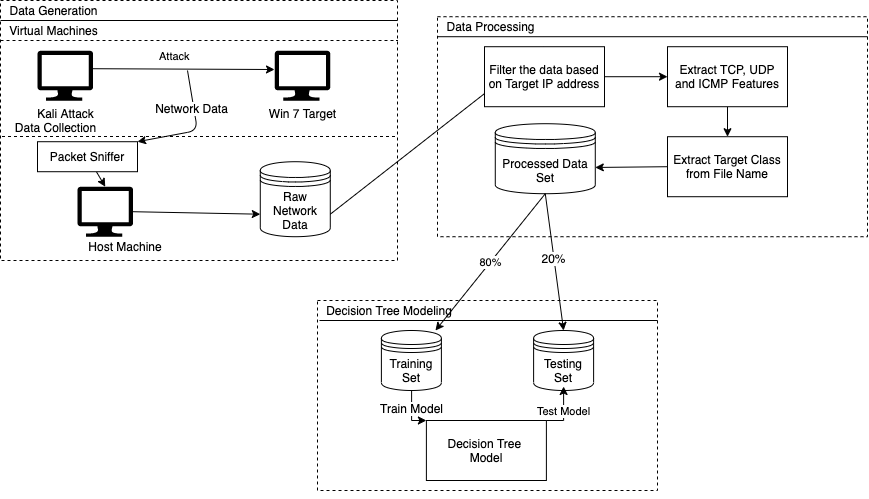
\includegraphics[scale = 0.45]{Images/Mainsystem.png}
\caption{Overall System Diagram}
\label{fig:osd}
\end{figure}

The systems diagram in Figure \ref{fig:osd} shows the 3 separate sections of the system and how they interconnect. Each module is built to the specifications defined in chapter \ref{chp:req}. The user may replace these \ depending on their specifications. 

\begin{itemize}
\item The data generation phase should allow the spinning of virtual machines, these virtual machines should then simulate an attack scenario. The network data from the attacks should then be collected by the host PC and stored as raw network data, the file name corresponding to the attack which has been made.
\item The data collection phase should process the data first by filtering IP addresses to only leave the packets the virtual machines have sent or received. Next, it must extract the TCP, UDP, and ICMP packets and their features. These packets should be collated every second to form the processed data set. The data will be labelled based on the file name. 
\item The decision tree modelling phase should split the dataset into training and testing sets and train a decision tree on the data. The model will be tested here and extracted for future use.
\end{itemize}

\section{Data Generation}\label{sec:datagen}
This part of the project is focused on the generation of raw network data. This will first be achieved by creating a virtualised network where the attacks will take place. The project uses a virtualised network, rather than a physical network made of hardware, because most attacks are designed to be harmful to the hardware that it attacks. Using a virtualised network allows the attacks to take place away from any hardware and leave no lasting effect. The plan for this module can be seen in Figure \ref{fig:dgd}.
\begin{figure}[H]
 \centering
 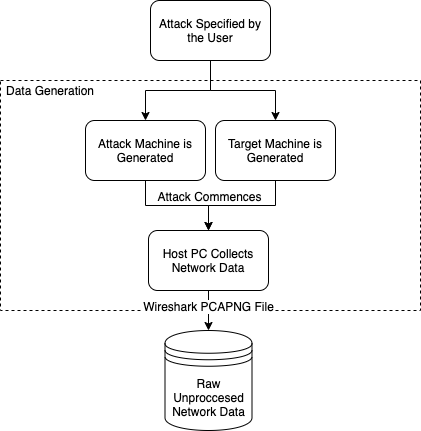
\includegraphics[scale = 0.5]{Images/datagen.png}
 \caption{Data Generation Diagram}
 \label{fig:dgd}
\end{figure}

\subsection{Virtual Machines}
\subsubsection{Virtual Machines Specification}

As seen in the systems diagram in Figure \ref{fig:osd} and in Figure \ref{fig:dgd} the project requires the generation of two virtual machines, namely the attack virtual machine and the target virtual machine. These two virtual machines become the virtualised network that will run the attack scenario.

The attack machine will run Kali Linux, a version of Linux that is tailored towards penetration testing and used widely in the cybersecurity community. This will mean a larger range of tools available for generating attack data and will allow future expandability of the project to contain a larger range of attacks. 

The target machine will run Windows 7, which makes up over 31\% of the operating system market share as of the time of writing \cite{osms}. Windows 7 is also commonly used within offices and is no longer supported by Microsoft as of January 14, 2020. The lack of support and the relatively high usage means that there are many unsecured PCs that could be attacked.

\begin{figure}[h]
 \centering
 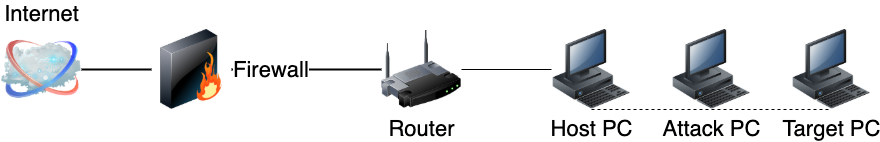
\includegraphics[scale = 0.45]{Images/VM_Network.png}
 \caption{Virtualised Network Diagram }
 \label{fig:vnd}
\end{figure}

The network diagram in Figure \ref{fig:vnd} shows the setup of the virtualised network. The host PC is connected to the router in some form, either by a wired connection or by a wireless connection. When the virtual machines are initialised they will connect to the router via a bridged connection. A bridged connection allows the virtual machines to be on the same network as the host PC and allows the host PC to communicate to the virtual machines.

\subsection{Packer}
Once the virtual machines have been created, as per the above specification, the next part requires the automatic generation of these machines. An open source tool called Packer will facilitate this. Packer was created to automate the creation of virtual machine images.\cite{pckr}. The user supplies two things, namely a template and a packer script.

A template for a virtual machine may be a pre-configured virtual machine, a separate image of this virtual machine or an ISO file, a file which containing an image of a CD containing the operating system to be installed to the virtual machine. 

A packer script is a configuration file which contain certain parameters which allow Packer to locate the virtual machine image, configure the image and build the machine. The configuration file contains three main sections, namely builders, communicators and provisioners \cite{pckr_doc}.

Packer uses a builder to build the virtual machine from some image. Packer can build virtual machines from VirtualBox\cite{pckr_doc}. This can be done directly from a virtual machine, from an Open Virtualisation Format (OVF) file or from an ISO file. This project will use the OVF file to create the machine because it allows greater possible portability of the project without the time sink of setting up virtual machines from scratch.

A communicator allows the host PC to communicate with the virtual machine to execute some commands. This can be done either via Secure Shell (SSH) or via Windows Remote Management (WinRM).\cite{pckr_doc} The host PC must be on the same network as the virtual machine for this to work as there must be a communication path between the virtual machines and the host PC.

Once a connection has been made, a provisioner is used to execute some actions in the virtual machine automatically. There are many provisioners available such as Shell, Ansible, Puppet and Chef among others.\cite{pckr_doc}. The project will use attacks which are written in shell scripts therefore requiring the use of the shell provisioner. Listing \ref{code:pckr_shell} form the packer documentation shows how the shell provisioner is used. A shell script, contained in the host PC, is specified and can run within the virtual machine.
\begin{lstlisting}[language = json, caption = Packer Shell Example, label=code:pckr_shell]
{
     "type": "shell",
     "script": "script.sh",
     "pause_before": "10s",
     "timeout": "10s"
}
\end{lstlisting}
Once a valid packer script has been written and a valid template exists, then packer can build the virtual machine by running the command:
\begin{verbatim}
 packer build template.json
\end{verbatim}
\subsection{Attacks}
Once the virtual machines are generated then attack scripts can be utilised to generate the required network data to build the dataset. 
\begin{table}[H]
 \caption{List of attacks}
 \label{table:attacks}
 \begin{tabular}{|c|c|l|}
 \hline
 \textbf{Attack}&\textbf{Tool}&\textbf{Command} \\
 \hline
 Normal& web-generator & \texttt{pyhton3 gen.py}\\
 \hline
 Syn Flood& Metasploit& \texttt{msfconsole -q -x "use auxiliary/dos/}\\
 &&\texttt{tcp/synflood;set RHOST IP;exploit;"}\\
 \hline
 FIN Flood&Hping&\texttt{hping3 --flood --rand-source -F -p }\\
 &&\texttt{PORT IP}\\
 \hline
 UDP Flood&Hping&\texttt{hping3 --flood --rand-source --udp -p }\\
 &&\texttt{PORT IP}\\
 \hline
 PSH \& ACK Flood&Hping&\texttt{hping3 --flood --rand-source -PA -p}\\
 &&\texttt{PORT IP}\\
 \hline
\end{tabular}
\end{table}
The attacks seen in Table \ref{table:attacks} will be used in the project. They were generated a few different techniques which were all present on the Kali Linux Distribution.

\subsubsection{Normal}
For any anomaly detection system to function correctly, the model must understand normal behaviour. Normal network usage can comprise many things. To best simulate normal network data, an open source python script called web-traffic-generator is used\cite{wtg}. A user on GitHub created this script, which sends HTTP requests to links that are found on the root-url in a pre-defined list of URLs. The script therefore aims to simulate a user browsing the Internet to allow the generation of organic, normal network data.

\subsubsection{SYN Flooding}
The first DoS attack that will be used is a synflood attack. The attack forms a general TCP connection with a TCP handshake. There are three key steps to the TCP handshake\cite{tcp_hand}:

\begin{enumerate}
\item The client sends a Synchronisation Sequence Number (SYN) informing the server the sequence number the connection will be made with

\item The server sends a response with the SYN-ACK flags set.

\item The client responds with the ACK flag set which enables a connection to happen
\end{enumerate}

The syn attack works by sending a large amount of SYN packets to the server. The server then has to keep the connection alive for each packet of these requests. This ensures that the server resources are all taken up with these requests\cite{syn}. An example can be seen in Figure \ref{fig:esfpr}.

\begin{figure}[H]
    \centering
    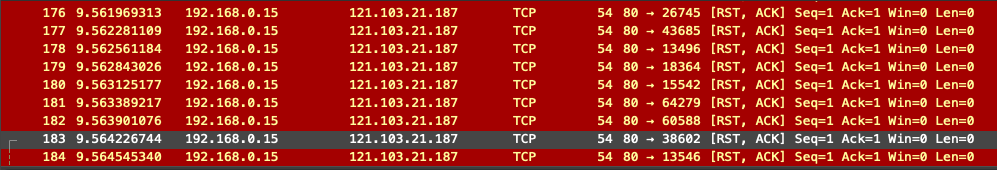
\includegraphics[scale = 0.4]{Images/synflood.png}
    \caption{Example synflood packets}
    \label{fig:esfpr}
\end{figure}

The tool used is Metasploit which is a penetration testing tool with an extensive list of exploits which can be used in a multitude of attacks.\cite{metasploit} 

\subsubsection{FIN Flood}
A FIN flooding attack is a DoS attack which floods the user with TCP packets which have the FIN flags set. The FIN flag indicates that the client is finished and there are no more packets to send. When a FIN packet is received the server and client have started a four-way termination handshake. This handshake starts with a FIN packet from the client, the server responds with an ACK packet and a FIN packet, which the client acknowledges. As the connection does not actually exist the FIN flood will cause the server to try to reset the connection and acknowledge the previous packet which ensures that the servers resources are again taken up. 

The tool used is Hping, which is another network security tool used mainly for penetration testing networks.\cite{hping}

\subsubsection{PSH \& ACK Flood}
When a server receives a packet with the ACK flag set, the server must respond with a confirmation that the packet was received successfully. When a server receives a packet with the PSH flag set, the server must process the information within the packet. Both flags means that the server has to do a lot of processing. When the processing is done the server will reset the connection to respond to the extra requests, all of this will take up large amounts of the server’s resources.

\subsubsection{UDP Flood}
A UDP flood follows a similar path to previous flood attacks. The attack aims to take advantage of how servers respond to UDP packets.\cite{udp} The server checks if any programs are listening on that port, if there are none, it sends an ICMP packet to inform the client that the port is closed. The server is therefore preoccupied with sending ICMP packets in response to the attack that most of the resources will not be available to legitimate users of the server.

\subsection{Data Collection}
After the network data can be generated there must be a way to collect the network data. For this the open source software known as Wireshark. Wireshark is a packet analyser which allows for the collection of packets which are being sent and are received on the network. Wireshark functions by putting the network interface into promiscuous mode, which allows it to see all of the incoming and outgoing network traffic.
 
\section{Data Processing}\label{sec:datapro}
This part of the project is directed around the parsing of the data amassed from section \ref{sec:datagen}, selecting useful features from the data and building a dataset. The raw network data which was generated in section \ref{sec:datagen} will be processed by, first filtering the packets to only contain those which arrived to or came from the virtual machines. Features are then extracted from these packets and are then collated so that the features are counted every second.

\begin{figure}[H]
 \centering
 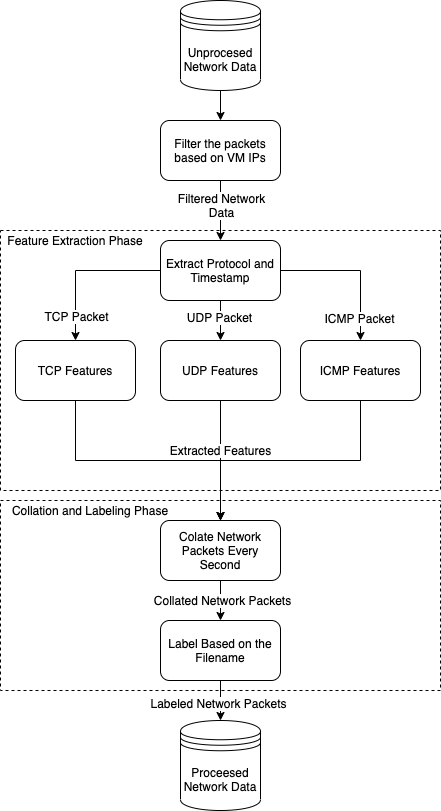
\includegraphics[scale = 0.5]{Images/datacollection.png}
 \caption{Data Collection Diagram}
 \label{fig:dcd}
\end{figure}
\subsection{Feature Extraction Phase}

Once the network data has been generated and collected with wireshark, it creates a PCAP Next Generation Dump (PCAPNG) File. This file type is the native file type for wireshark and contains all the network data generated from an attack. Wireshark collects the network data of the Host PCs network. As this network will contain noise from other machines connected to it, the data must first be filtered. Since an intrusion detection system will mainly run on the target PC, the filtering will only include packets that are sent to and received from the target machine. Wireshark allows filtering network data using DisplayFilters \cite{filters}. 

\begin{verbatim}
 ip.addr == 192.168.0.15
\end{verbatim}

The filter above will only keep packets that came to or arrived from the target machine. This can be achieved by setting a static IP for the target machine image so that the IP address will never change. This means that all the packets in the collection will be from the attack and will thus will limit noise. While it can do this in wireshark, it does not automate it. For the automation of the process, a library needs to be used to extract the packets and store the important pieces of data into a CSV file. 

\subsubsection{Pyshark}
Pyshark is an open source python library which wraps tshark\cite{pyshark}, tshark is a terminal-based version of wireshark which can allow for parsing out network data from PCAPNG files. This project uses pyshark version 0.4.2.9 which was released on Aug 11, 2019.

\begin{lstlisting}[language = python, caption = Pyshark Example Code, label=code:pyshrk]
import pyshark
self.cap = pyshark.FileCapture(input_file="normal.pcapng", 
 display_filter =filter)
# Write the packets
for packet in self.cap:
\end{lstlisting}

The Code seen in Listing \ref{code:pyshrk} shows an example of reading a network file. Once these packets are read then they can be looped through one by one and the features extracted. From here they can all be stored as a CSV file or stored in an array to be manipulated later.

\subsection{Feature Selection}

One of the most essential parts of building a machine learning algorithm is feature selection. Feature selection refers to the act of choosing features in your dataset that best contribute to the target class. Performing good feature selection will allow a much cleaner model, which is less prone to overfitting and improves accuracy.\cite{feat_select}.

\begin{table}[H]
 \centering
 \caption{List of Features to be Extracted Initially}
 \label{table:features_init}
 \begin{tabular}{|c|c|}
 \hline
 \textbf{Feature}&\textbf{Data Type}\\
 \hline
 Timestamp & Date \& Time \\
 \hline
 Protocol & Integer\\ 
 \hline
 Source Port & Integer\\
 \hline
 Destination Port & Integer\\
 \hline
 TCP Finish Flag & Binary Value\\
 \hline
 TCP Synchronise Flag & Binary Value\\
 \hline
 TCP Push Flag & Binary Value\\
 \hline
 TCP Acknowledge Flag & Binary Value\\
 \hline
 TCP Urgent Flag & Binary Value\\
 \hline
\end{tabular}
\end{table}

The features seen in Table \ref{table:features_init} are the features which are initially extracted from the network data. For a DoS attack, it is important to know what type of protocol was used and what flags were set, from this the DoS attack can be determined. However, on their own these features are not enough as a single packet gives no context about what is happening within the network, to better distinguish what is going on within the network the packets must be collated within a time frame to lend some context to the packet.

In their paper, P.Sangkatsanne et al. \cite{SANGKATSANEE20112227} found 12 features that best differentiated the attacks they used. They did this using information gain, as seen in the literature review.

\begin{table}[h]
 \centering
 \caption{List of Features from P.Sangkatsanne et al.}
 \label{table:features}
 \begin{tabular}{|c|c|}
 \hline
 \textbf{Feature}&\textbf{Data Type}\\
 \hline
 Number of TCP packets & Integer \\
 \hline
 Number of TCP source ports & Integer\\ 
 \hline
 Number of TCP destination port & Integer\\
 \hline
 Number of TCP finish flag & Integer\\
 \hline
 Number of TCP synchronise flag & Integer\\
 \hline
 Number of TCP push flag & Integer\\
 \hline
 Number of TCP acknowledge flag & Integer\\
 \hline
 Number of TCP urgent flag & Integer\\
 \hline
 Number of UDP packets & Integer\\
 \hline
 Number of UDP source port & Integer\\
 \hline
 Number of UDP destination port & Integer\\
 \hline
 Number of ICMP packets & Integer\\
 \hline
\end{tabular}
\end{table}

The features seen in Figure \ref{table:features} are the features which are extracted from the network data, these features are aggregated every 2 seconds. The paper claims that these features will be able to sufficiently classify DoS and Probe attacks. As this paper will mainly focus on DoS attacks, these features should differentiate between them.

The timestamp seen in Table \ref{table:features_init} will be used to collate the network packet features into one second data points. 
\subsection{Collation and Labeling Phase}
Once the features of each individual packet are extracted they must be collated, and the features seen in Table \ref{table:features} extracted from them.
\subsubsection{Pandas}
The Python Data Analysis Library (Pandas) is a python library that deals with data manipulation and analysis. Pandas will take some data from a data type such as a CSV or a list and create a Dataframe. A dataframe is a 2D labelled data structure that resembles a spreadsheet \cite{pandas_docs}. Dataframes allow easier indexing by time and can quickly apply functions to an entire column instead of looping through each data point in the dataset.

Here pandas can collate the network data into dataframes which contain the packets in a particular second. From here, it can apply operations to extract the features from the packets, as in Table \ref{table:features}. These can then be written to a CSV containing the previous attack data to generate a dataset.
\subsubsection{Labeling}
Each network file is stored with the name of the attack, this filename can be used to label the attacks once the network packets are processed.
\section{Data Modeling}
This part of the project is focused on using the processed data from section \ref{sec:datapro} to train a machine learning model. The processed network data will be split into training and test data to ensure no overfitting, and a model is trained from this data. From the literature review, the consensus is that a decision tree model would perform best for Intrusion detection.
\subsection{Scikit Learn}
Python has many packages to use for machine learning but the one which supports the most algorithms is scikit learn. scikit learn is a python library which implements multiple machine learning algorithm including a decision tree algorithm by implementing the CART algorithm. scikit learn is very simple to use and is compatible with pandas so the network data can be read and can train the classifier. This project uses scikit learn version 0.22.2 released on Mar 4, 2020.
\begin{lstlisting}[language = python, caption = Decision Tree scikit-learn Example, label=code:skit]
from sklearn import tree
X = [[0, 0], [1, 1]]
Y = [0, 1]
clf = tree.DecisionTreeClassifier()
clf = clf.fit(X, Y)
\end{lstlisting}
The code seen in Listing \ref{code:skit} is an example implementation of a decision tree classifier taken from the documentation \cite{scikit}. The code is easy to implement and creates a good classifier that can be used in production.\cite{scikit_prod}. 


%--------------------------------------------------------
% Implementation
%--------------------------------------------------------
%--------------------------------------------------------
% Implementation
%--------------------------------------------------------
\chapter{Implementation}
This chapter will cover the implementation of each three sections of the project as outlined in the requirements and design chapter. It discusses the decisions made for each section and any changes from the design that were made. This chapter will also document any additions made. This chapter will also include the testing process.

\section{Development Approach}

As previously discussed the project should contain 3 separate sections which should be developed prior to the project being implemented under one roof. Therefore, the project utilised an agile development strategy. Agile development allows iterative development where the requirements can change during the development of the project. As agile is used the implementation plan will comprise first implementing the ‘Essential’ sections of the project, these sections can later be revisited and less essential sections can be added.

\subsection{Implementation Plan}

An essential part of any implementation is planning prior to it. As the most important section is the data generation section of the project, this will be done first to ensure that at least some data can be extracted to be used in future sections of the project. The data however must be processed before it can apply to a machine learning model and the data processing will be implemented next. Finally, the data modeling section of the project can be implemented.

To ensure that the project succeeds, any requirement which was given a ‘Essential’ importance in Table \ref{table:req} must be implemented before moving on to the next section. Once all the essential requirements have been implemented, and the project works to a satisfactory level, any remaining requirements given the ‘Important’ importance level can be implemented. Finally, any requirement given the ‘Desirable’ importance level will be implemented, given enough time.
Through this method each part of the project can be split into blocks. When a block of work is complete, its resembles a part of the project which is complete and functioning. 
\subsubsection{Block Plan}
\begin{enumerate}[
    leftmargin=*,
    label={Block \arabic*.},
    ref={Block (\arabic*)}]
    \item Implement all Essential requirements for the Data Generation project section, namely OS.1,OS.4, DG.1-2, DG.4-8. 
    \item Implement all Essential requirements for the Data Processing project section, namely OS.2, DP.1-4. 
    \item Implement all Essential requirements for the Data Modeling project section, namely OS.3, DM.1.
    \item Implement all Important requirements for the project, namely OS.5, DG.3-4, DM.2-3.
    \item Implement other requirements with either a ‘Desirable’ importance or any other requirements not yet implemented.
\end{enumerate}

The project must be done in the order above, ensuring that the project functions correctly at each block and that testing can be done to each block as they are implemented.

\subsection{Programming Language}
The programming language chosen for this project is Python 3.7.4. This is primarily because of my personal familiarity with the language. Coding in a familiar language makes writing code initially easier and also makes debugging code easier. In conclusion, the adoption of a familiar programming language makes programming simpler and quicker.

Python also provides compatibility over a broad variety of operating systems without having to modify the code at all. The code to be written can run on Windows, Unix and Mac satisfying requirement UP.7.

Python also has a large amount of open source libraries to complement the already comprehensive standard library. This means that Python can be moulded with libraries to do a large plethora of things. In this project libraries will launch packer, deal with network data and train a model.

\section{Virtual Machines}
As seen in Figure \ref{fig:vnd} a simple virtual network needs to be automated. This simple network will require an attack machine and a target machine to be generated automatically and connect to the same network, so as to be visible to each other. This will however not represent a usual network, I have made the network simple for prototyping purposes. The same ideas presented here can be altered relatively simply to represent a more complex network with more nodes.

\subsection{Virtual machine images}
To create the virtual machine images, a virtual machine to image must first be created. Creating virtual machines using the VirtualBox GUI is relatively simple, and the process is similar for both systems. An in-depth guide can be seen in the VirtualBox documentation \cite{vb_docs}. 

\subsubsection{Virtual Machine Creation}
Following the step-by-step guide seen in the documentation, the two virtual machines were created. The Kali Linux attack machine was allocated 2GB of RAM and a 20GB Hard Drive, as the machine need not be powerful to execute these basic threats. The Windows 7 target machine was allocated 1GB of RAM and a 32GB Hard drive, the increased hard drive size is because of the space which Windows needs to be installed. The 1GB of RAM should be enough to maintain the operating system as no programs need to be launched during the attack.

Once the machine is launched VirtualBox requests an .iso file to boot from which should contain the relevant files to install an operating system. 

For Kali Linux the .iso file is freely available from their website \cite{kl}. Windows 7 however is not a freely available operating system, therefore a product key was purchased and the .iso file downloaded from their website \cite{w7}. Following the relatively simple step-by-step setup wizards to install both operating systems the machines can now be configured.

\subsubsection{Setting a Static IP}
As discussed in the design section, each virtual machine must have a static local IP address, to allow the attack and target machines to communicate and to allow filtering of packets later on. Altering the static IP address is different for both operating systems. 

\textbf{Kali Linux} - For Kali Linux the static IP can be changed from the command line. First the file  \texttt{/etc/network/interfaces} needs to be altered. Inside that file these lines were added
\begin{verbatim}
    auto eth0
    iface eth0 inet static
    address 192.168.0.14/24
    gateway 192.168.0.1
\end{verbatim}
This alters the ip address of the \texttt{eth0} interface to 192.168.0.14, the ip address which will identify the attack machine. Once this alteration has been made the networking service must be restarted.
\begin{verbatim}
    sudo systemctl restart networking.service
\end{verbatim}
\begin{figure}[h]
    \centering
    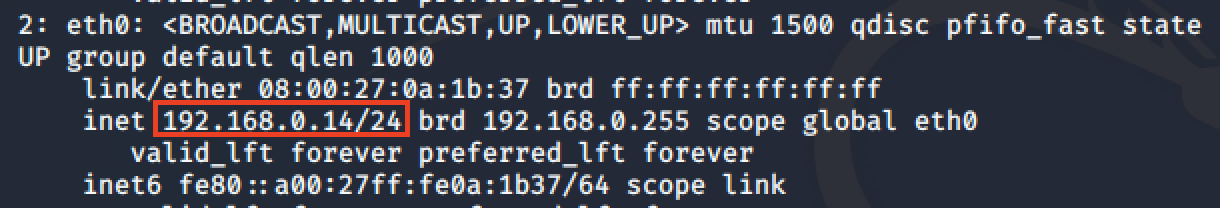
\includegraphics[scale=0.65]{Images/ip.png}
    \caption{IP Configuration for Attack Machine}
    \label{fig:ipfa}
\end{figure}
When the service has restarted, the IP should have changed as in Figure \ref{fig:ipfa}. This IP will stay as the IP address of the machine when the machine will be restarted/exported.

\textbf{Windows 7} - For Windows 7 the static IP can be changed from the Control Panel. First the relevant section of the control panel should be accessed by Start Menu > Control Panel > Network and Sharing Center > Change adapter settings. From here the Local Area Network interface  Internet Protocol Version 4 (TCP/IPv4) properties are accessed, the IP address is then changed to include the static IP address. The static IP for the target machine will be 192.168.0.15. Once saved the IP address of the target machine will have been altered as seen in Figure \ref{fig:ipft}.
\begin{figure}[h]
    \centering
    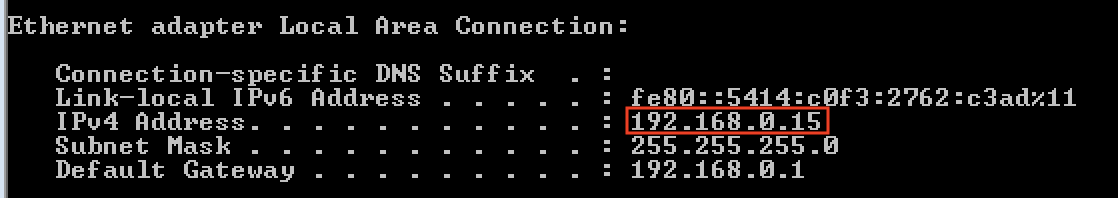
\includegraphics[scale=0.7]{Images/ip7.png}
    \caption{IP Configuration for Target Machine}
    \label{fig:ipft}
\end{figure}

\subsubsection{Target Machine Configuration}
The target machine represents a vulnerable machine which an attacker may take advantage of. As this is the case for the Windows 7 machine the Windows Firewall must be turned off. This can be done by accessing the Windows Firewall section of the Control Panel and turning the windows firewall off. This will allow the machine to become vulnerable to DoS attacks.

\subsubsection{Exporting the Virtual Machines}
Once the machines have been fully configured they must be exported. Virtual machines can be exported to Open Virtualisation Format (OVF) Files via Virtualbox, the full instructions can be found in the Virtualbox documentation \cite{vbovf}. Both the attack and target machines will be exported to OVF files to be used in the project. These images are however rather large, totalling almost 15GB for the two images. This will cause problems if these machines are to be distributed as part of a package.

\subsubsection{Bridged Network Connection}
Setting up a bridged network connection is simple. From the Virtual Machine Settings > Network page the network can be changed from NAT network to a Bridged Network. This involves choosing the interface on the host PC to bridge. 

\subsection{Packer Scripts}
A packer script, as discussed in the design section, is used to build and run a virtual machine from an image. For both the attack machine and target machine a separate JSON script file is needed, and since the attack shell script has to be specified in the provisioners section of the script, this means that each attack will need its own script. To counteract this the name of the attack can be specified on the launching of the program and a python library can alter the attack script.

Packer.py is a library which allows interacting with packer from Python \cite{packerpy}. Once installed the library can be used from within the program to build the template and run the script. Building the template in the program allows many alterations to be made to the script before run-time without writing and saving a new script.

\begin{lstlisting}[language = python]
p = PackerExecutable(self.executable_path)
\end{lstlisting}

Before Packer.py can run the library needs to find the location of the packer executable, without this it cannot run the scripts. Unfortunately the packer executable file is stored in different places depending on computer and operating system. Because of this in the program the user must specify the location of the packer executable. The project will allow the user to specify it within a config file.

\subsubsection{Attack Script}
\begin{lstlisting}[language = python, caption = Attack Script, label=code:atts]
attack_template = """{{
"builders": [
    {{
    "type"                  : "virtualbox-ovf",
    "vboxmanage": [
             ["modifyvm", "{{{{.Name}}}}", "--bridgeadapter1", "{interface}"]
                   ],
    "source_path"           : "{machine}",
    "vm_name"               : "attack",
    "boot_wait"             : "30s",
    "ssh_host"              : "{ip}",
    "ssh_port"              : 22,
    "ssh_username"          : "{username}",
    "ssh_timeout"           : "20m",
    "ssh_password"          : "{password}",
    "ssh_skip_nat_mapping"  : "true"
    }}
],
"provisioners":
[
    {{
    "type": "shell",
    "script": "{attack}"
    }}
]
}}
"""
\end{lstlisting}

The code contained in Listing \ref{code:atts} shows the attack script template, from here the format function can be used to fill the template in and the packer build function can launch the virtual machines.

The attack contains a builder section, which specifies how the virtual machine is to be imported and booted. A provisioner section, which runs the attack script on the virtual machine. Finally, the packer.py build function will run the script. The specifics of the template are defined below: 
\begin{itemize}
    \item \texttt{type} - Defines the builder that will be used. Here the virtualbox ovf image builder is used.
    \item \texttt{vboxmanage} - Defines any vboxmanage commands which are to be run before boot. This is used to change the network interface name.
    \item \texttt{source\_path} - Specifies the location of the virtual machine image. The user specifies this path in the config file.
    \item \texttt{vm\_name} - Specifies the name of the virtual machine when imported.
    \item \texttt{boot\_wait} - Specifies the time in seconds that packer waits for the machine to fully boot. This is essential as if packer doesn’t wait it cannot ssh into the machine.
    \item \texttt{ssh\_host, ssh\_port, ssh\_username, ssh\_password, ssh\_timeout} - specifies the information needed to allow packer to ssh into the virtual machine. All the information here is specified by the user in the config file except for the ssh port and the ssh timeout. These should stay the same.
\end{itemize}
\subsubsection{Target Script}
The target script is set up a little differently than the attack script. The template seen in Listing \ref{code:ttts} contains only a builder. There is no provisioner section as there is no need to run any programs on the target machine while the attack is going on. The rest of the template is very similar to the attack script except the \texttt{boot\_wait} acts as a timer which allows the virtual machine to continue running for a specified time before packer turns off the virtual machine. This will be utilised to allow the machine to stay on and wait until the attack has finished.
\begin{lstlisting}[language = python, caption = Target Script, label=code:ttts]
template = """{{
"builders": [
    {{
    "type"                  : "virtualbox-ovf",
    "vboxmanage": [
                ["modifyvm", "{{{{.Name}}}}", "--bridgeadapter1", "{interface}"]
                  ],
    "source_path"           : "{machine}",
    "vm_name"               : "target",
    "communicator"          : "none",
    "guest_additions_mode"  : "disable",
    "virtualbox_version_file": "",
    "boot_wait"             : "{time}s"
    }}
]
}}
"""
\end{lstlisting}

\section{Development}

The three sections of the project were developed as separate python packages. The project uses Python packages as a way of organising modules within a project. A folder is created, all files within that folder are a part of the package and an \texttt{\_\_init\_\_.py} tells python which files and classes to import from the  folder. In this project, as there are three sections, there will be three packages each dealing with an individual section. The three packages can then be imported into a main file which can run the program from the command line. 

The file structure should therefore contain three folders, each implementing a separate section of the project. The file structure of the finalised project can be seen below:

\dirtree{%
.1 geranium.
.2 data\_generation.
.3 attacks.
.3 capture.
.3 virtual-machines.
.3 traffic-gen.
.3 datagen.py.
.3 \_\_init\_\_.py.
.2 data\_processing.
.3 data\_parser.py.
.3 data\_processor.py.
.3 \_\_init\_\_.py.
.2 data\_modeling.
.3 data\_modeling.py.
.3 \_\_init\_\_.py.
.2 intrusion\_detection.
.3 ids.py.
.3 \_\_init\_\_.py.
.2 geranium.py.
.2 config.yaml.
.2 setup.py.
.2 requirements.txt.
.2 README.md.
}

The following section will describe the implementation of each section and the design changes which were made to either improve the project or to satisfy a requirement.

\section{Main Program}

\texttt{geranium.py} is the main file of the project, this is the user's main input into the project. The project will work like a typical command line interfaces. The user will specify a sub-command and some arguments. From these the program should call the relevant functions from the relevant packages and execute them with the arguments provided. 

Prior to this however the user must have all relevant third-party libraries installed. The running of geranium.py does not depend on any third-party libraries, however the three packages require third-party libraries. To ensure the user can install them easily a \texttt{setup.py} file is written. This file allows a python package to be installed, and the relevant dependencies installed. The dependencies are placed within \texttt{requirements.txt} file. This file is read and passed into the \texttt{setup()} function as an array. This array tells the python interpreter which dependencies are needed for this package to work. The user may run \texttt{python3 setup.py install} to install the package and all the dependencies. Once this is done the user may begin, so long as they have Packer and Virtualbox installed.

The native argparse and sys python modules are used to parse the arguments given by the user on the command line, define sub-commands which the user can run to access features of the program and read the command line arguments provided by the user. Before the user can access any of the features of the program, they must first write a config file. The config file is a YAML file which contains relevant pieces of information which the program will use when running an example can be seen in Appendix \ref{app:conf}. For instance the locations of both attack and target machines will be stored within the file. The \texttt{pyyaml} module is used to parse the YAML file. Once parsed the file becomes an easy to manipulate dict object. From here the relevant pieces of information are parsed and stored as global variables to be utilised if relevant.

Once the user is fully setup, they may begin. The gerainum.py file is an executable file so it can be run directly from the command line. The user simply needs to type \texttt{./gerainum.py}. This will print out a help message detailing to the user the sub-commands or options available to them. The help message may also be accessed by executing the file with the \texttt{-h} flag. The sub commands also have help messages which may be accessed both by running with no arguments or by running with the \texttt{-h} flag. When an invalid sub command is given the user is presented with the help message.  On execution of a valid command the program will take the name of this command and execute a function of the same name found within the class. These functions themselves also have parsers within them to parse the arguments into the relevant packages. There are five main commands the user can execute. 

\textbf{Generate} - The generate command will run the data generation section of the project. The user must first have 2 valid virtual machine images to launch and an attack to simulate. The user must also fill in the relevant sections of the config file. Once filled in, the data generation can be executed by running the command. 
\begin{verbatim}
    ./geranium.py generate <attack name> <path/to/attack.sh>
\end{verbatim}
This will run for the allotted time as defined in the config file and will generate a CSV with features as defined in \texttt{data\_processing/data\_parser.py}. The user may also generate normal network data. Since the web-traffic-generator \cite{wtg} is used here there is no need for virtual machine to boot up or for an attack script to be launched. The command is therefore:
\begin{verbatim}
    ./geranium.py generate normal
\end{verbatim}
Generating normal data requires only the time to be specified within the config file.

\textbf{Process} - The process command will run the data processing section of the project. The PCAPNG files which were generated by the generate command can be processed here. Again the user must alter the config file specifying the path they wish to write to and a filter to be used on the packets. Once these have been specified the user can process data by executing the command:

\begin{verbatim}
    ./geranium.py process <attack_name> <path/to/network_data.pcapng>
\end{verbatim}

\textbf{Model} - The model command will run the data modelling section of the project. The dataset the user has generated may train a decision tree classifier. The config file must contain the path that the user wants to output the model, and the classes in the dataset. Once these have been specified the user can generate a model by executing the command:
\begin{verbatim}
    ./geranium.py model <path/to/dataset.csv>
\end{verbatim}

\textbf{IDS} - The project also contains a rudimentary system for running an intrusion detection system. This will take the model which the project generated and use it on live network data to show if there is an attack commencing on the computer. The user can specify the model to be used in the config file and can run the intrusion detection system by executing the command:
\begin{verbatim}
    ./geranium.py ids
\end{verbatim}

\textbf{Clearvms} - On exit all the relevant folders for the virtual machines should have been removed, but sometimes if the user forces the exit of the program or an error occurs within the virtual machines the folders may not be removed by the \texttt{onexit} handler. The \texttt{exit\_handler()} function applies two vboxmanage \texttt{unregistervm} commands to delete the machines, and any related files. Next the \texttt{rm} command is used to remove the \texttt{packer\_cache} and \texttt{output-virtualbox-ovf} directory. If this is the case, the user can run the clearvms command to clear the folders.
\begin{verbatim}
    ./geranium.py clearvms
\end{verbatim}

\section{Data Generation}
The \texttt{data\_generation} package provides the classes and functions required to generate network data from a virtualised network attack scenario. Generating data is the most essential section of this project and was the first package which was implemented. The \texttt{datagen.py} file implements the packer scripts allowing the spinning up of virtual networks. The file also implements automatic network capture.
\subsection{Attacks}
The \texttt{attacks} directory contains the attacks which were used to generate the network data in this project. There are 4 attacks contained within this directory as defined in Table \ref{table:attacks}. The main issue with all these DoS attacks is that they are designed to be run in the command line and exited by the user. This would mean that the shell script would force the attack machine to run forever. This was counteracted by introducing a timeout. The timeout command is a Linux command which can introduce a timeout to a command. It will end the program if it is still running within that time. The command to execute a synflood attack for 10 minutes will be:
\begin{verbatim}
    timeout 10m msfconsole -q -x "use auxiliary/dos/tcp/synflood
                                  ;set RHOST 192.168.0.15
                                  ; exploit;"
\end{verbatim}
    
The commands seen within Table \ref{table:attacks} were all written with the same timeout as the synflood attack seen above and stored within the \texttt{attacks} directory. When these attacks are defined by the user in the command line, they are written to the provisioners section of the template file. The shell script will then run on the virtual machine, once Packer had successfully made a ssh connection into the machine, until the timeout finishes, the command exits and the shell script exits. This will free up Packer to close the machine and clear up.

\subsection{Data Generation}
The main file in this package is the \texttt{datagen.py} file which contains the \texttt{DataGen()} class. This class contains all the functions required to execute the requirements of this section.

The \texttt{\_\_init\_\_} function is a constructor function in python which is called when an object of this class is created. All the relevant configurations from the config file are passed into the object and are assigned to variables within the class. The function next checks to see whether the user has specified the generation of normal network data. If they have, the program will first generate a new thread to launch the \texttt{start\_network\_capture()} function. The function launched wireshark from the command line by using the below command. This command when executed by the program will start wireshark on the interface defined after the \texttt{-i} flag. Wireshark will run for the duration specified in the configuration file and will save the file in the \texttt{capture} folder 
\begin{lstlisting}[language = python]
    command = "wireshark -k -i wlp3s0 -a duration: " 
              + str(self.time) +
              " -w capture/" 
              + self.attack + 
              ".pcapng"
    os.system(command)
\end{lstlisting}
Next the function will run the web-traffic-generator \cite{wtg} located within the \texttt{traffic-gen} folder. 
\begin{lstlisting}[language = python]
    os.system("timeout " 
              + str(self.time) + 
              " python3 data_generation/traffic-gen/gen.py")
\end{lstlisting}

The timeout command is used here to ensure that the script runs only for the specified time within the config file. The web-traffic-generator runs indefinitely and so needs to be exited when no longer needed. The path must be from the root directory as the command line which the user is running \texttt{geranium.py} is in the root directory. Once the time has expired, the user will have a file which contains simulated normal network usage.

If the user specifies an attack to be run the program will first run the \texttt{run\_vms()} function. The function launches the virtual machines in separate threads. Two threads are launched by calling \texttt{create\_attack\_machine()} and \texttt{create\_network\_target()} in separate threads. This is essential as the building of the two virtual machines should be done in parallel to ensure that both machines will be online together and would not have had to wait for the other machine to build and exit before it can start. 

The \texttt{create\_attack\_machine()} function first declares the packer object by passing the Packer executable path. The template seen in Listing \ref{code:atts} is declared and the relevant configurations which were passed from the main program are written into the template; the variables are written into the sections which contain \texttt{\{VAR\_NAME\}} in Listing \ref{code:atts} using the \texttt{attack\_template.format()} function. Finally, the template is passed into the packer \texttt{build()} function. Along with the template the force flag is also passed into the build function. This allows packer to build the same image multiple times even if there are remnants in the packer cache.  

While the virtual machines are being built, the main thread waits until the attack machine is online before it collects network data. The main thread will execute a while loop which runs the \texttt{ping\_vm()} function. This function will ping the attack IP address with a single packet, when the machine does not respond the function will return False. If the machine responds then the function will return True. The while loop will break when the function returns True. The program will then wait 30 seconds for Packer to ssh into the computer and start running the attacks. Once 30 seconds have elapsed the main thread will execute the \texttt{start\_network\_capture()} function and start collecting network data. 

\subsubsection{Collecting Network Data}
As discussed in the original design for the project, the idea was to use wireshark to collect the network data and to use pyshark to parse the network data into a dataset. This was how the project was implemented for a long period, however collecting network data and parsing the useful features separately seemed like a convoluted way to generate data. Because of this, the implementation of \texttt{start\_network\_capture()} was altered. Instead of launching wireshark the program will import the \texttt{DataParser()} class from the \texttt{data\_processing} package. To stay true to the modularity of the project all the code to implement the packet sniffing and feature extraction was implemented within the \texttt{data\_processing} package rather than in the \texttt{data\_generation} package. The parser will therefore be explored in more detail in the data processing section of the implementation. 

\subsubsection{\_\_init\_\_.py}
The \texttt{\_\_init\_\_.py} file is used by python to identify a package. An empty file will show that the \texttt{data\_generation} folder is a package. If any classes are imported within the \texttt{\_\_init\_\_.py} file they become available to the user on import of the package. For this package the \texttt{\_\_init\_\_.py} file imports the DataGen class:
\begin{lstlisting}[language = python]
    from .datagen import DataGen
\end{lstlisting}

\section{Data Processing}
The \texttt{data\_processing} package provides the classes and functions required to process any generated network data. The \texttt{data\_processing.py} file contains the original design of the data processor using pyshark. The \texttt{data\_parsing.py} file contains the network collection and feature extractions in one and replaces wireshark in collecting network data. Even though the data parser is used within the data generation section of the project, it is still implemented within the data processing section to keep the modularity of the project while also allowing the user to alter a single file to implement their own features rather than worry about changing code in more than one place. The implementation of \texttt{data\_processing.py} is still included in the command line just in case the user wishes to use wireshark to have a store of the raw network packets and wishes to extract features from it.

\subsection{Processing data from raw packets}
The \texttt{data\_processing.py} file contains the classes and functions to process network data. The file will take a pcapng file from wireshark and extract the features seen in Table \ref{table:features_init} using pyshark. Then using pandas the packets will be collated, and the features seen in Table \ref{table:features} can be extracted. This follows the diagram seen in Figure \ref{fig:dcd}. 

The \texttt{\_\_init\_\_()} function serves only to take the relevant sections from the configuration file, like in \texttt{datagen.py}. The function also declares an empty list called \texttt{packets} where the initial extracted features are to be stored. 

The function \texttt{read\_packets()} imports the capture file into pyshark, as in the example seen in Listing \ref{code:pyshrk}. Here a filter can be passed from the configuration file if the user requires it. Next the function loops through every packet within the capture file and extracts the protocol and timestamp from then. Next it checks which headers are available from the packets and extracts the relevant features from them and writes them to a list.

Next the function \texttt{collate\_packets()} takes these extracted features and creates a dataframe object from them. The dataframe uses the timestamp column as an index and the \texttt{datafrm.groupby(pd.Grouper(freq=’1s’)):} function generates a list of dataframes where the packets have been grouped with a frequency of one second. This allows functions to be applied to the entire dataframe rather than having to loop through every packet. Applying the \texttt{value\_counts()} function to the protocol column will give the number of packets of each protocol. To retrieve the number of distinct source ports and destination ports a separate dataframe is created containing only the protocol and either the source or destination port, from there the \texttt{value\_counts()} function was applied for both TCP and UDP protocols, which returned a list of the unique ports and the length of the list was taken. As the flags are a binary feature, calculating the sum of the values will return the number of times that each flag is set in the packets.  

\subsection{Data Parser}
The \texttt{data\_parser.py} file contains the classes and functions required to collect and process network data. The file will sniff packets using the Scapy module and extract the features seen in Table \ref{table:features_init}. Then using pandas the packets will be collated, and the features seen in Table \ref{table:features} can be extracted. This follows the diagram seen in Figure \ref{fig:dcd}. 

The initial idea was to use the native sniff ability of pyshark to incorporate the network data collection into the \texttt{data\_processing.py} file. However, there were issues around threading and stability which are explored in more detail in the Implementation Issues section later. Because of this issue the Scapy package was used. Scapy is a python package which is mainly used to manipulate packets \cite{scapy}. The package has a native \texttt{sniff()} command which is used in \texttt{data\_parser.py} to collect network data. In the \texttt{\_\_init\_\_()}, along with the normal declarations of configurations, the hexadecimal equivalents for the flags are defined. From these values, the flags can be identified from the packets.

\begin{lstlisting}[language = python]
    self.FIN = 0x01
    self.SYN = 0x02
    self.RST = 0x04
    self.PSH = 0x08
    self.ACK = 0x10
    self.URG = 0x20
\end{lstlisting}

In the function \texttt{sniff\_packets()} the \texttt{sniff()} function is called, specifying the function which will decode the incoming packet, the time it should run for and any filters to apply to the packets. If no interface is specified to the function, it collects the network data along all interfaces, this is the setting which is used here. The \texttt{process\_packet()} function takes a packet as an argument and extracts the relevant features as defined in Table \ref{table:req}. This is a very similar process to the code within the \texttt{read\_packets()} function in the previous section. As before, when the features are extracted they are stored within a list to be processed later. The \texttt{collate\_packets()} function remains unchanged from \texttt{data\_processing.py}. The \texttt{sniff\_packets()} function is called within the \texttt{start\_network\_capture()} function in \texttt{datagen.py}.

\section{Data Modeling}
The \texttt{data\_modeling} package provides the classes and functions required to build a decision tree model from the processed dataset. The \texttt{data\_modeling.py} file is the main file within the package and implements a tree classifier from the \texttt{sklearn} library.

\subsection{Decision Tree Classification}
The \texttt{data\_modeling.py} file contains the \texttt{DataModeling()} class. The \texttt{\_\_init\_\_()} function takes the relevant sections from the configuration file. The dataset is imported into a pandas dataframe using the \texttt{read\_csv()}. The set is then split into two separate dataframes where one contains all the features and the other contains the target classes.

From here the tree is trained by calling the \texttt{train()} function. The function first splits the dataset into a training set and a test set using the \texttt{train\_test\_split()} function from \texttt{sklearn.model\_selection} with an 80:20 split. The decision tree’s \texttt{fit()} function is then called to train the tree using the training set. The tree uses the gini impurity defined in Equation \ref{eq:gini}

The \texttt{test()} function allows the model to make predictions based on the test set. From these predictions the accuracy, recall and precision can be calculated using functions from the \texttt{sklearn} library. These functions implement Equations \ref{eq:acc}, \ref{eq:precision} and \ref{eq:rec}. Cross validation is also applied to test the model.

Finally the \texttt{export\_tree()} function will allow the model to be exported using the \texttt{joblib} library to export the variable as a .joblib file. This file can later be utilised in an intrusion detection system.

\section{Repository Overview}
This section will detail the third party repositories used in the project. These are all specified within the \texttt{requirements.txt} so they can be installed within the \texttt{setup.py} file.
\begin{itemize}
    \item \texttt{pyyaml} - Used to prase the configuration file.
    \item \texttt{pandas} - Used to collate network data.
    \item \texttt{scapy} - Used to collect network data and extract features.
    \item \texttt{pyshark} - Used to extract features from wireshark pcapng files.
    \item \texttt{sklearn} - Used to train a decision tree model.
    \item \texttt{joblib} - Used to export the trained decision tree into a file.
    \item \texttt{packer.py} - Used to interface with the packer command-line tool and automatically build and run virtual machines.
\end{itemize}

\section{Implementation Issues}
As with any project the implementation of the project presented some issues which had to be overcome to ensure a working piece of software. These issues were generally centered on automating the building of virtual machines and the automatic collection and extraction of network data. Most issues had a relatively simple solution and required no alternations to the original design.
\subsection{Pyshark Threading Issues}
Pyshark’s native live interface capture function was initially to be used to collect network data from the attacks and the features extracted at the same time as they come in. However when pyshark is called from within a thread, it would cause an exception and the program to crash. Upon researching the error I found multiple GitHub issues, some of which still open, relating to this error. An example open issue can be found at \url{https://github.com/KimiNewt/pyshark/issues/303}. 

Pyshark also crashed rather frequently because of crashes in tshark, I could not find a solution to this error but an example of an open issue with the same problem can be found at \url{https://github.com/KimiNewt/pyshark/issues/232}. Often the only way to solve the issue was to restart the computer. Because of these issues Pyshark was deemed not stable enough to be used in the project. It was instead replaced with the Scapy package as detailed in the Data Processing section. This required a slight alteration in feature extraction to accommodate the new packet structure.
\subsection{Virtual Machine Images}
As detailed above, the virtual machine images both total to about 15GB. These files are far too large to distribute with the package and they can not be committed onto GitHub. To resolve the issue the path to the virtual machines were simply added onto the \texttt{.gitignore} file. This file tells Git not to commit the folder onto the repository. 

The user can make virtual machine images themselves and may want to do so to better resemble their network. However, for basic network attacks the images used in testing should be fine. However, the images cannot be supplied as the target image runs Windows 7, and requires a licence. While they may have been stored on a cloud service to be downloaded if two Linux systems were used, this is unfortunately not possible with the testing images because of the licensing.

\subsection{Modeling issues with non-numeric classes}
As the data generation and processing section of the project was done prior to the data modeling section of the project all the target classes were stored in the dataset as strings. This caused issues because sklearn does not support non-numeric classes. The initial solution involved manually altering the class names, using find and replace. This sufficed for initial testing however is not a long-term solution. 

For a longer term fix the \texttt{preprocessing} module from sklearn is used. The label encoder function will take a list of classes and encode each class with a number. The numbers given to them can uniquely identify the classes and sklearn will train a model using the data without altering the dataset manually. 

\subsection{Target Operating System}
Most Penetration testing applications involve the usage of a Windows XP target system. This is because of its relatively high usage compared with its age and lack of support from Microsoft. There is a 30 day trial period for running Windows XP without a valid licence key, and periodically the XP system will stop functioning and request a product key before booting. 

Also, the user may need to run a script on the target machine to facilitate more complex threats. Issues around setting up Windows Remote Management and the inability to set up SSH in the target machine meant that packer could not access the machine as it was running. Because of this Windows 7 was used as it is still not supported by Microsoft but the OpenSSH server can be installed on the machine. This was done in this project but the SSH facility was not used.

\subsection{Issues with Bridging the Network}
The virtual machines in the project utilise a bridged network connection. This means that the interface must be specified for virtual box to bridge the connection. This presents issues for the portability of the project. When the project is moved to a different computer and imported, Virtualbox may not find an interface of the same name to bridge.

The error seen in Figure \ref{fig:vmerror} will happen when the machines are imported. This error will not allow the machine to be launched until the error has been rectified by the user. The solution was to use VBoxManage. VBoxManage is a VirtualBox command-line tool which can interface with VirtualBox. VBoxManage commands may be executed from a Packer script.

\begin{lstlisting}[language = json, caption = Bridged Connection Solution, label=code:bcn]
"vboxmanage":[
                ["modifyvm", "{{.Name}}", "--bridgeadapter1", "en0"]
             ],
\end{lstlisting}

\begin{figure}[h]
    \centering
    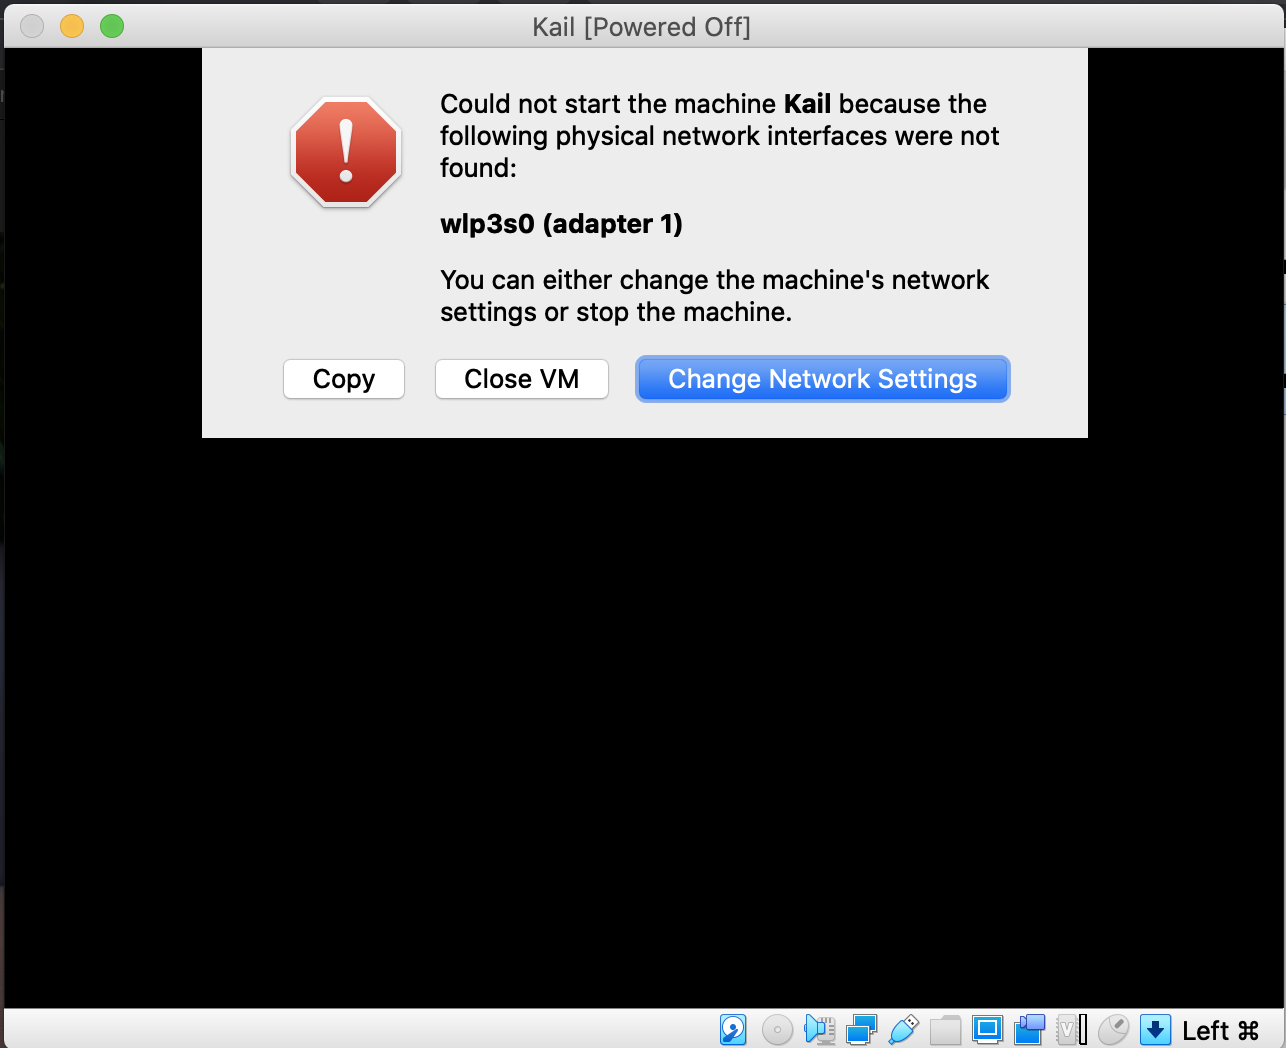
\includegraphics[scale=0.5]{Images/vm_error.png}
    \caption{The Bridged Connection Error}
    \label{fig:vmerror}
\end{figure}

The code seen in Listing \ref{code:bcn} is the Packer implementation of a VBoxManage command. This command tells the virtual machine to set the interface of the bridged adapter to \texttt{"en0"} which is the interface of my laptop. I do this before the virtual machine boots so this will change the adapter before the error can happen. The interface for the virtual machines can be specified in the config file.










%--------------------------------------------------------
% Testing and Evaluation
%--------------------------------------------------------
\chapter{Evaluation and Testing}\label{chp:tes}
Testing is an essential part of the project as it for allows unforeseen issues to be detected. The system will first be tested in its entirety to ensure it functions correctly, this will be done in parallel with development. Unit tests will also be written for each section to ensure the development of functioning modules. The system must also meet the requirements set out in Chapter \ref{chp:req} and as such will be tested based on these requirements. This chapter will also evaluate the final developed project both in its overall state and in its three separate parts. This chapter will also assess the limitations of the project.

\section{Full System Testing}
Full system testing involves testing the system in a use case scenario. In this case the system will be tasked with generating normal network data and network data from the attacks found in the \texttt{attacks} directory. The data is automatically processed and stored to a CSV file. 
The Full system utilises a network which resembles that of \ref{fig:vnd}. The attack machine being a Kali Linux machine and the target machine being either a Windows XP or Windows 7 machine, as the switch to windows 7 happened early on but not before some data was generated. The normal network data was generated on the Host PC connected to the network. The noise from other devices connected to the network in normal network data generation serves to help simulate the more unpredictable nature of normal network data.

Throughout development the parts of the system which were deployed were utilised to either, generate or process data to be used in the next part of the development. Because of this the full system deployment was done during the Implementation plan detailed within the Implementation chapter.

The dataset generated consisted on 20,379 rows, the dataset mainly consisted of normal network data. The normal network data was run for four hours, this was done in the hopes of reducing the number of false positives. The rest of the data was generated in different chunks between 10 minutes and 30 minutes. This dataset is utilised thought testing to train models.

This scenario is built to represent a typical usage of the tool. The model generated from this scenario will be able to detect different types of threats. The full scenario uses the attacks from Table \ref{table:attacks}:
\begin{enumerate}
    \item Generate normal data for 4 hours
    \item Generate attack data for 10 - 30 minutes
    \begin{enumerate}
        \item synflood
        \item udpflood
        \item finflood
        \item pshackflood
    \end{enumerate}
    \item Process data (done automatically in the generate command)
    \item Train model with the generated data
\end{enumerate}
Unit tests were written to test each step of the above scenario, the unit test for the normal data generation is given in Listing \ref{code:unt}:
\begin{lstlisting}[language = python, caption = Normal Data Unit Test, label=code:unt]
def test_normal_generation(self):
        """
        Test that normal data can be generated
        """

        data_generation.DataGen("normal",
                                None,
                                None,
                                10,
                                None,
                                None,
                                None,
                                None,
                                None,
                                "data.csv",
                                None)
        
        time.sleep(1)
        self.assertTrue(os.path.exists("data.csv") and os.path.getsize("data.csv") > 0)
\end{lstlisting}

These tests utilise the native \texttt{unittest} python package. The tests can be run in the command line and can be executed individually by using the \texttt{python -m unittest test\_module.TestClass.test\_method} command. These unit tests check to see if the file which is supposedly generated by the package has been generated and contains text. 

Finally a large test was written which executes the relevant commands from the command line to run the above scenario fully. The config file must be first configured and then the commands are executed sequentially. Finally culminating in the model being generated.
\subsection{Time to Generate Normal Data}
The unit test for generating normal data is used to test the speed of setting up, running and processing normal network data. The unit test was run 5 times, each time taking the time needed to run the unit test native to the \texttt{unittest}. The First unit test can be seen in Listing \ref{code:unt}, this will run Normal network generation for 10 seconds.
\begin{table}[H]
	\begin{minipage}{0.4\linewidth}
        \centering
        \caption{Results of Unit Test 1}
        \label{table:unittest1}
        \begin{tabular}{cc}
         \textbf{Test No.}&\textbf{Time (s)}\\
         \hline
            1&	11.029\\
            2&	11.043\\
            3&	11.026\\
            4&	11.03\\
            5&	11.034\\
            \hline
            \textbf{Average} & 11.0324
        \end{tabular}
	\end{minipage}\hfill
	\begin{minipage}{0.6\linewidth}
            \centering
            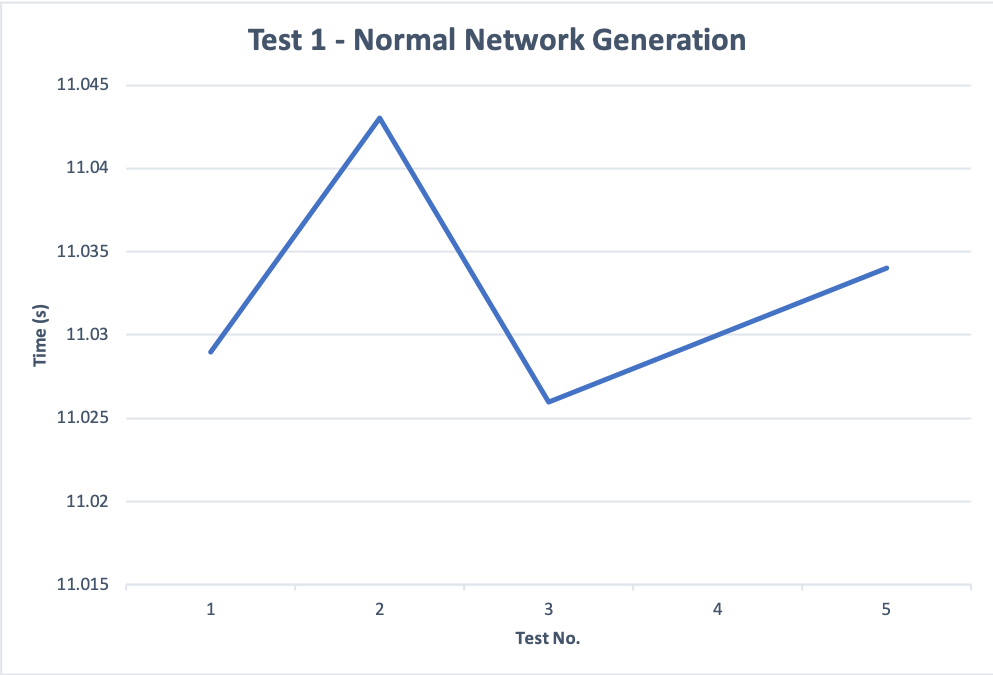
\includegraphics[scale = 0.4]{Images/Results/unittest1.png}
            \captionof{figure}{Graph of Unit Test 1}
             \label{fig:unittest1}
	\end{minipage}
\end{table}
As can be seen in the results from Table \ref{table:unittest1} the running time for generating 10 seconds worth of normal network data is, on average 11 seconds. As the web-traffic-generator is running for 10 seconds this means that collating the network packets and extracting the features from them takes approximately 1 second. The graph in Figure \ref{fig:unittest1} again shows that as the tests were completed the time taken remained consistent. This data generation will generate 10 rows of data in the dataset as the network packets are collated per second.
\subsection{Network Data Collection}
In extension to unit test 1, unit test 2 was built to test the amount of time required to collect network data and extract the required features from them. The test was run for differing times to see how increasing the amount of network data would alter the time taken to process it.
\begin{table}[H]
\centering
\caption{Results of Unit Test 2}
\label{table:unittest2}
\begin{tabular}{ccccc}
 \textbf{Generate Time (s)}&\textbf{Test 1 (s)}&\textbf{Test 2 (s)}&\textbf{Test 3 (s)}&\textbf{Average (s)}\\
 \hline
    1 & 2.067& 2.062& 2.045& 2.058\\
    10& 11.159& 11.203& 11.217& 11.193\\
    50& 52.165& 51.971& 51.691& 51.94233333\\
    100& 102.557& 102.782& 02.423& 102.5873333\\
    200& 206.891& 203.733& 204.192& 204.9386667\\
    600& 612.432& 614.682& 615.499& 614.2043333\\
\end{tabular}
\end{table}
\begin{figure}[H]
    \centering
    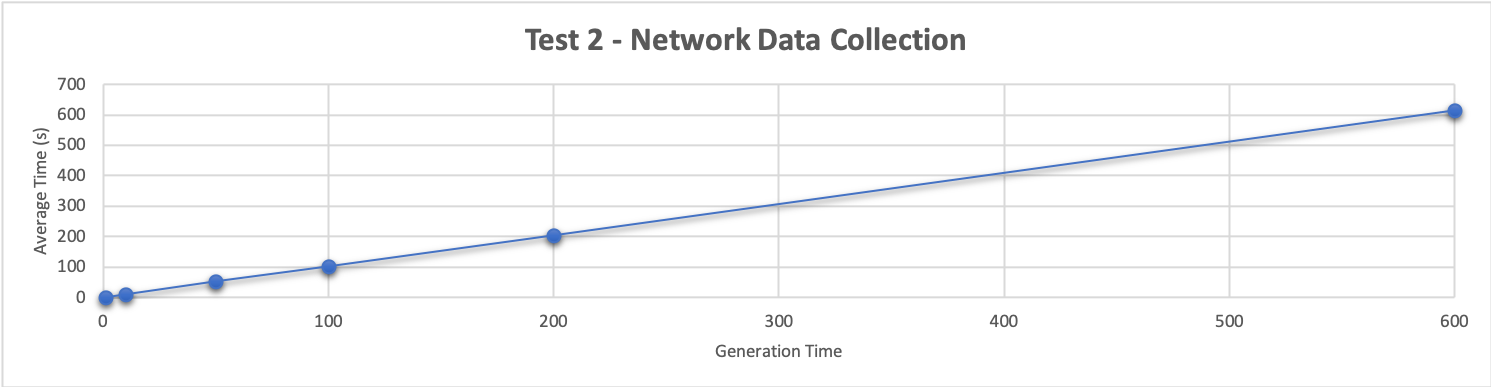
\includegraphics[scale = 0.5]{Images/Results/unittest2.png}
    \caption{Graph of Unit Test 2}
     \label{fig:unittest2}
\end{figure}
As can be seen by the results in Table \ref{table:unittest2} and the graph in Figure \ref{fig:unittest2}, as the time increases and the amount of network data increases, the time required to process the data also increases linearly. This makes sense as processing this data is done with pandas dataframe, which supports array programming where methods can be applied to a dataframe as a whole rather than to the individual features, which reduces time.

\subsection{Generating Attack Data}
The unit test for generating attack data will spin up two virtual machines and run a synflood attack for one minute before shutting down the machines, extracting the relevant features and removing all virtual machine files. The  \texttt{test\_attack\_generation()} function within the test file will execute this scenario.
\begin{table}[H]
\centering
\caption{Results of Unit Test 3}
\label{table:unittest3}
\begin{tabular}{cccc}
    \textbf{Test No.}& \textbf{Target (min)}&\textbf{Attack(min)}& \textbf{Full Scenario (min)}\\
    \hline
    1& 1:39	&2:39& 4:51\\
    2& 1:41	&2:43& 4:27\\
    3& 1:44	&2:49& 5:16\\
    4& 1:30	&2:17& 4:15\\
    5& 1:35	&2:10& 5:04\\
    \hline
    \textbf{Average} & 1:37 & 2:31& 4:46
\end{tabular}
\end{table}
As can be seen in the results from Table \ref{table:unittest3} the generation of the attack machine tended to take on average 1 minute 37 seconds while the target machine took, on average almost an extra minute to launch. This is in part due to the absence of a communicator or provisioner in the target machine, leaving packer to do less configuration. This was also due to the lower relative size of the target machine image in comparison to the attack machine. The target machine was 4.16GB while the attack machine was 10.85GB. 

The average execution time for the one minute data generation was 4 minutes 46 seconds. 2 minutes 30 were taken up on average launching the machine, about 30 seconds were taken for the attack machine to boot and a minute was taken for the attack leaving about 46 seconds the program took to power off machines and clear the virtual machines. 

Data generation in this form often resulted in less than the expected 60 rows of data. This is due to the fact that sometimes there are no packets to or from the target machine, especially before or after the attack runs and as such Scapy does not collect any packets. 

\subsection{Decision Tree Modeling}
This unit test was used to train the decision tree with the generated network data from the full system testing. The system will train five decision tree models and will run the relative metrics. A maximum depth of 5 was used during testing.
\begin{table}[H]
\centering
\caption{Results of Unit Test 4}
\label{table:unittest4}
\begin{tabular}{ccccc}
    \textbf{Test No.}&\textbf{Time (s)}& \textbf{Accuracy}& \textbf{Precision}&	\textbf{Recall}\\
    \hline
    1& 3.421& 99.8\%& 99.4\%& 99.3\%\\
    2& 3.697& 99.9\%& 99.7\%& 99.4\%\\			
    3& 4.081& 99.9\%& 99.9\%& 99.4\%\\
    4& 3.721& 99.9\%& 99.8\%& 99.9\%\\
    5& 3.856& 99.7\%& 99.7\%& 99.9\%\\
    \hline
    \textbf{Average} & 3.755& 99.8\%& 99.7\%& 99.3\%\\
\end{tabular}
\end{table}
As can be seen in Table \ref{table:unittest4} the decision trees modeled from the dataset which was generated during full system testing. The cross validation scores for each decision tree are seen below.
\begin{verbatim}
    Tree 1 - [0.99828263 0.99705594 0.99926398 0.9990184 0.99386503]
    Tree 2 - [0.99828263 0.9968106 0.99926398 0.9990184 0.99386503]			
    Tree 3 - [0.99828263 0.99705594 0.99926398 0.9990184 0.99386503]
    Tree 4 - [0.99828263 0.9968106 0.99901865 0.9990184 0.99386503]
    Tree 5 - [0.99803729 0.9968106 0.99901865 0.9990184 0.99263804]
\end{verbatim}
The decision trees have an accuracy and an average cross validation score  of 99\% which shows that the decision tree makes accurate decisions based solely on the data which has been generated by the user. It also shows that decision trees are a good classifier to use in this scenario. The decision tree also has a 99\% Recall and Precision which indicates that the decision tree has a low level of False negative and false positives which indicates that the generation of data through the virtual machines had no adverse effect to the modeling. On average the time taken to train the decision tree, test and extract the tree is just under four seconds. This is due to the dataset containing threats which are easily differentiated. 

\begin{figure}[H]
    \centering
    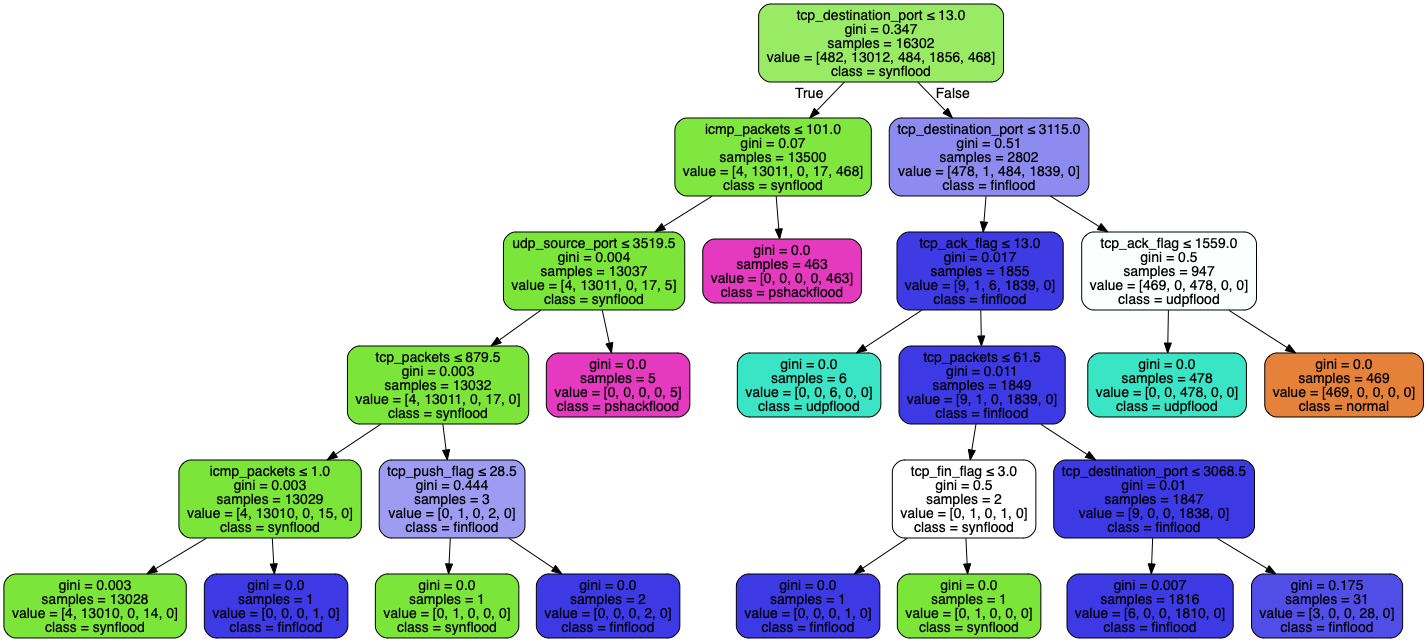
\includegraphics[scale=0.3]{Images/Results/tree.png}
    \caption{Decision Tree}
    \label{fig:dectres}
\end{figure}

The decision tree which was generated in the full system testing can be seen in Figure \ref{fig:dectres}. As can be seen the tree is relatively compact and as such can be considered to be not overfit. Overfitting can also be ruled out by looking at the metrics, which used cross validation and other methods to ensure the randomness of the test set. Therefore without defining a max\_depth the tree does not overfit the data despite certain sections of the tree in \ref{fig:dectres} containing nodes which define the same class.

The project was successful in generating a large scale dataset to be used within a decision tree model, however collating network data by the second means that the amount of data which is able to be generated is dependant on the time which the system can run for. For instance receiving 1 million rows of data for a particular attack will require the system to run for one million seconds which translates to just under 12 days. The workload can be reduced by running the program on multiple machines or by utilising different features. The project therefore is reliant on the amount of time which the user can spare, while 10 minutes seem appropriate for these attacks it may take longer if the differences between attacks are less clear.

The project only focuses on collecting network data from the machines, as detailed in the background section this is sufficient for threats such as DoS and Probe attacks but is not sufficient for R2L or U2R threats as these alter system files within the computer. The project does not collect any system logs at the moment but the collection of system logs can be automated in the target machine by using Packer provisioners.
\section{Requirement Based Testing}
Requirement based testing involves testing the created system based on the requirements set within Chapter \ref{chp:req}. All system requirements have been detailed below however not all other requirements have been detailed due to the subjective nature of a few of them.
    \begin{tabularx}{\textwidth}{|c|X|X|}
    \caption{Implemented Requirements}
    \label{table:irq}\\
    \hline
     \textbf{Code}& \textbf{Requirement Details}&\textbf{Implementation Details}\\
     \hline
     OS.1  & The system should automatically generate a virtualised network and simulate an attack & The system can generate two virtual machines from images and can run shell scripts on the attack machine to attack the target.\\
     \hline
     OS.2 & The system should collect the data from the simulated attack, the program should extract the relevant features and process the data into a dataset & The \texttt{data\_processing} package allows the user to both process raw network packets or process live network data from the \texttt{data\_generation} package. \\
     \hline
     OS.3 & The system should train a decision tree model to differentiate between different DoS attack & The user is able to specify the dataset when calling the \texttt{model} command. \\
     \hline
     OS.4 & The system should allow users to write their own attacks and to be able to run them in the virtual network & The user is able to specify the path and name of their attack when calling the \texttt{generate} command.\\
     \hline
     OS.5 & The system should allow the user to implement their own versions of each section to meet their requirements & The source code uses open source packages and so can be supplied on Github. The code is written in three separate packages which can be altered or and swapped.\\
     \hline
     DG.1 & The program must be able to automatically import 2 or more virtual machines from images, power on the virtual machines and run programs on each virtual machine. & The system can take two virtual machine images, specified in a config file, and generate two virtual machines from packer templates.\\
     \hline
     DG.2 & The virtual machines must connect to the same network and be accessible to both the host computer and each other & The images are set to connect to a bridged network and the packer template uses a vboxmanage command to ensure the interface is correct.\\
     \hline
     DG.3 & The virtual machines must power off after data collection is finished and they must delete themselves and their files. & The machines are powered off by Packer and the files removed either by the exit handler or the \texttt{clearvms} command. \\
     \hline
     DG.4 & The virtual machines must have the same IP address, they can be later identified from these IP address & This is set on each individual operating system.\\
     \hline
     DG.5 & The program must collect the network data which moves between the virtual machines & This was originally achieved by launching wireshark but is currently implemented by the \texttt{sniff()} function provided by the \texttt{scapy} library.  \\
     \hline
     DG.6 & The capture should run only when the attack starts and must stop when the attack finishes & The capture only starts when there is a response from the attack machine when pinged.\\
     \hline
     DG.7 & The program must also simulate normal network data and collect this data & The user is able to generate normal network data by running the web-traffic-generator using the \texttt{generate normal} command\\
     \hline
     DG.8 & The network packets must be saved to a file with a readable name & As wireshark is not used anymore the processed network data is now stored directly within the dataset. The path of the dataset is specified by the user. \\
     \hline
     DP.1 & The network packets need to be read from section \ref{sec:datagen}. & As the processing now occurs as soon as the network data comes in this is no longer necessary. However the previous implementation using \texttt{pyshark} is included. \\
     \hline
     DP.2 & The initial features, as in Table \ref{table:features_init} need to be extracted from the network data. & This is done by extracting the features from each packet and storing them within an array. \\
     \hline
     DP.3 & The packets need to be collated per second and the features, as in Table \ref{table:features}, need to be extracted & The packets are converted to a dataframe and then collated.\\
     \hline
     DP.4 & The packets need to be saved to a comma separated value (CSV) which will contain all the threats. & The generated dataframes are written to the csv path specified within the configuration file.\\
     \hline
     DM.1 & The model must be trained by data which was generated from the virtual machines & The user can specify the path when executing the \texttt{model} command\\
     \hline
     DM.2 & The model should be able to predict attacks with a >90\% accuracy. This is due to the KD99 dataset generating >90\% accuracy models \cite{SANGKATSANEE20112227} \cite{Peddabachigari} \cite{bouzida}. & This is achieved by the dataset the program was tested with.\\
     \hline
     DM.3 & The model should have a high amount of true positives and a small amount of false positives, a common issue in anomaly intrusion detection is a high level of false positives. & This is achieved by the dataset the program was tested with.\\
     \hline
     RE.1  & The project should run without error & This is achieved through good programming practice and testing.\\ 
     \hline
     RE.2 & Each section of the project should run without error independently & This is achieved in the project, each section is able to be run independently.\\
     \hline
     UP.1 & The program should be straightforward to use & The program uses sub commands and arguments in the command line, each command contains help screens and the config file is well commented. \\
     \hline
     UP.2 & The user should be able to use the system for their own uses without needing to understand how the code was implemented & The help screens and command line interface should allow usage of the program without extensive knowledge.\\
     \hline
     UP.3 & The project should not require special hardware to run, however may require a base spec to run sufficiently well. & 3GB of RAM and around 60GB of hard drive space is needed for the virtual machines to load. A dual core Intel i5 processor was used in testing however an i3 should be sufficent.\\
     \hline
     UP.4 & The process of data generation should be automated and should not require the user’s input & This has been achieved.\\
     \hline
     UP.5 & The project should run at a reasonable speed and not cause the system to crash & This was achieved on a 2017 Macbook pro with 8GB ram and a dual-core i5 processor.\\
     \hline
     UP.6  & The project should run on Windows, Mac and Unix Systems & The software has been tested on a Mac and an Ubuntu machine.\\
     \hline
\end{tabularx}
The project implemented all of the essential requirements and most of the important requirements and most desirable requirements were kept in mind and implemented in the project.
\subsection{Limitations}
The project has a few limitations due to the time spent on development or due to the scope of the project.
\begin{itemize}
    \item The project in its current state is only able to collect network data and does not collect any system logs
    \item The project only utilises two virtual machine images for a virtualised network as seen in Figure \ref{fig:vnd}.
    \item The system can take a long period of time to generate enough data for the user.
    \item The project does not aim to write any novel attacks. These must be written by the user if they require it.
\end{itemize}
\section{Project Evaluation}
The data generation section of the project provided the largest amount of issue, from designing to testing. The design was difficult due to my relative lack of understanding around the subject in the beginning. A large amount of time in the early times of the project were spent trying to fully understand the scope of this section and how it was to be implemented. Even when a design was fully realised, in practice changes were made to streamline the system as my knowledge of the area grew. The section as a whole works very well but took up a large chunk of time to develop, this was due to the time required to fully test a system. As can be seen from the results in this chapter a single one minute test can take up to five minutes, often when testing functionality which is due to happen after the machines close testing took several hours. This meant that this particular block took a much longer time than any other development block. Testing for the data generation block was done over the period of a few days due to the relatively small amount of attacks which had to be trained for. The smaller amount of threats and the relatively large amount of packets generated, by nature of the DoS attack, meant that the testing was rather straightforward. But as the attacks get more complex and more data is required then more time will be taken to generated enough data.

The data processing of the project was originally developed without issue, simply taking the data which had been generated previously and extracting the relevant features from it. However after much thought this was changed to allow it to be Incorporated with the data generation module. This reduced the time required to generate data and made a lot more sense. The design developed due to an increased experience with network data extraction modules in python allowing me to develop the packet sniffer in the program rather than using another third party piece of software which the user needs to install. The collection and processing of network data is fast, often taking around fourteen seconds to collate ten minutes of packet data. Testing involved simply running the code for different lengths of time to understand how the length of time taken to collect and extract data changed as the length of time data was required for changed also. Using an open source library allows the user to alter the features which they extract to better suit their needs.

The data modeling section of the project was developed with little issue. The section utilised the \texttt{sklearn} package to both implement the project and test it. The library had a large range of functions and modules to use during the implementation of the project. The library which allowed the development of this section to be completed and tested quickly. The models which were generated during testing had high accuracy and precision meaning that they could be utilised as very efficient intrusion detection systems, though the development of such intrusion detection system is beyond the scope of the project. 

The overall system was developed after the three sections above were completed. This me to ensure that the essential sections of the project worked and were developed properly before tying the sections together. Originally as these modules were separate packages they were imported into files much like libraries and their functions called when needed. However this did not make much sense as the functions rarely return anything and the user would have to develop a program to call and run the functions. Due to this the command line interface was developed in the hopes that the project would become more usable. The command line interface utilises simple syntax to allow the user to easily navigate the project. The sub commands are fairly self explanatory and the help pages indicate to the user exactly how they should use the sub-commands. A setup.py file was also written to ensure that the user can easily install dependencies.

Scheduling the development of the project was highly dependant on results from testing. The project could not continue until data had been generated for instance. This often meant than sometimes the time needed to develop a module was underestimated. While suitable time was found to develop the project more time should have been allocated to the blocks so as to ensure they were finished before moving on.

The agile software development methodology allowed me to develop the project in a much better way. When the project had started developing the ideas which now form a crucial part of the project such as the network collection or command line interface were not originally part of the design. The agile methodology allowed me to learn from development and return to previously designed sections of the project and alter them. Overall the project successfully created a model from a dataset formed of generated network data from an automated virtualised network.




%--------------------------------------------------------
% Conclusion and Future Work
%--------------------------------------------------------
\chapter{Conclusion and Future Work}
The initial concept for the project was to develop a tool that can automate the generation of network data to apply to an anomaly-based intrusion detection system. The project therefore first concentrated on research around the fields of intrusion detection systems and virtualisation, while not much pertinent material was found about the latter, at least in the cybersecurity field, there were a substantial collection of papers found which related to the use of machine learning techniques in intrusion detection systems, therefore a vast chunk of time was saved by studying existing research. From this research, a decision tree classifier was utilised in the project. However, the larger job of automating the generation of data had limited research around it and so had to be designed from scratch. The project has realized all of its objectives, principal of which was developing the capacity to generate datasets from automated virtualised network data. 

The research into automating virtualised networks reveals that I may use the networks in a cybersecurity setting to reliably generate network attack data. The user can write attack scripts to run on this virtualised network to generate network data, the network data will build a personalised dataset. The report also shows that this network data can then be applied to an anomaly intrusion detection system. This project provides a usable framework to allow the user to develop more complex and sophisticated tools from the datasets generated.

The program was packaged into a straightforward command based interface to be utilised by the user. The user does not require high-level technical knowledge to generate data or a model.

One particular future development avenue would integrate the project into a more complex system to generate novel attack data. The system would implement a novel technique to attack a network, the attack could then be executed on the automated system once they are run. A large amount of network data would be generated which could bolster network defences against more devious threats.

Automating the extraction of the system logs from the target machine would open up the possibilities of generating network data from a wider range of exploits such as the Canary Red’s Atomic Tools. These attacks would assume that access had already been made to the target machine and would run relevant attacks and extract system log data to detect these threats.

Using system logs would involve an alteration to the data collection and data processing process currently in place. The system might have to collect more network features and would have to parse system logs into the dataset despite there not being a one-to-one mapping between network data and systems logs.

Since this project is aimed at developing a system which any person could feasibly use, future research could work on developing the ability to alter the amount of machines on the network, and to alter the systems which run upon the network. 

Implementing ensemble learning techniques instead of a decision tree could be considered in the future. This will help reduce the risk of over-fitting from a single decision tree. This project’s scope, however, did not touch upon the different machine learning algorithms which could be used in place of the decision tree however the user could alter the data modelling section of the project if they wished to change the classifier.

The project has fulfilled all of its aims, chief of which was developing the ability to generate datasets from automated virtualised network data. These aims have allowed the development of a framework of which to build upon. There are multiple different avenues with which to move the project forward, the most compelling of them would be based on developing tools which can be used alongside the project to develop novel attack data, much like the Metasploit attacks used in this project. 

%--------------------------------------------------------
% Ethics
%--------------------------------------------------------
\chapter{Professional and Ethical Issues}
During the development of any project there are certain ethical standards which must be upheld. Since this project is almost entirely software based, great care was taken to ensure that all aspects of the project fell strictly within the guidelines of the British Computer Society Code of Conduct \cite{bcs}. Following the code of conduct ensures that I created the project in a legal and socially appropriate manner.

Under the 'Duty to Relevant Authority' section of the code of conduct, rule 3.e. states that:
\begin{quote}
    You shall NOT misrepresent or withhold information on the performance of products, systems or services (unless lawfully bound by a duty of confidentiality not to disclose such information), or take advantage of the lack of relevant knowledge or inexperience of others \cite{bcs}.
\end{quote}

In accordance with section 3c of the code, no claims were made in this report or in any documentation which aimed to mislead the reader/user or overestimate the ability of the program. This allows a potential user to be sure of what the program does before downloading or deciding to develop upon it. 

Under the 'Public Interest' section of the code of conduct, rule 1.b states that:
\begin{quote}
    You shall have due regard for the legitimate rights of Third Parties \cite{bcs}.
\end{quote}

As the project involves the use of many third-party libraries and software. Where any third-party libraries and programs have been used, I have made this clear in this report and in development in accordance with the code. Any work within the project is my own except where explicitly stated otherwise. The project relies heavily upon operating systems running within the virtual machines. The use of all operating systems was licensed when appropriate and the testing images were not provided in line with such licensing.

Under the 'Professional Competence and Integrity' section of the code of conduct, rule 2.d. states that:

\begin{quote}
    You shall ensure that you have the knowledge and understanding of Legislation and that you comply with such Legislation, in carrying out your professional responsibilities  \cite{bcs}.  
\end{quote}

The most pertinent law around cybersecurity in the United Kingdom is the Computer Misuse Act of 1990 \cite{cmua}. The law aims to define under what circumstances someone may be charged with a cybercrime. The law states that 
\begin{quote}
     A person is considered guilty of an offence if they cause a computer to perform any function with intent to secure access to any program or data held in any computer, the access they intend to secure is unauthorised; and they know at the time when they cause the computer to perform the function that that is the case \cite{cmua}.
\end{quote}
 The project does not violate the computer misuse act due to the computer being a set of virtual machines running on the users computer, the access is therefore authorised. The intent of the project is very clearly defined to be furthering the development of intrusion detection systems and all attack suites provided are open source third party frameworks.
 
Any software developer must ensure that any project undertaken abides by the Data Protection Act 2018 \cite{dpa}. As the act only applies to personal data which is kept by the developer the act does not necessarily apply here. However to ensure that all user data is protected any data generated within the project is stored locally, at a location designated by the user. No unnecessary information such as the users name, address and date of birth is taken. 

While this project makes use of user scripted network exploits and hacking. This falls within the definition of ethical hacking, which unlike regular hacking is legal. Ethical hacking is defined as the hacking of a system, with the express knowledge of the systems owner, in the hopes of either testing defences or finding vulnerabilities within the system\cite{ethhak}. This project utilises hacking tools to exploit a pre-configured system, with pre-defined vulnerabilities, hoping to generate network data to build defences for that system. This is done with the knowledge of the systems owner and to better equip that system with defences. 








%--------------------------------------------------------
% Bibliography
%--------------------------------------------------------
\bibliographystyle{unsrt}
\bibliography{references}
\addcontentsline{toc}{chapter}{\numberline{}References} 

%--------------------------------------------------------
% Appendices
%--------------------------------------------------------
\appendix
\renewcommand\chaptername{Appendix}
% \renewcommand*{\thechapter}{A.\arabic{chapter}}
\titleformat{\chapter}[display]
  {\centering\normalfont\Large\bfseries}
  {\MakeUppercase {\chaptertitlename\ \thechapter}}
  {0pt}
  {\MakeUppercase}
\chapter{User Guide}
\section{Prerequisites}
You must have packer and virtualbox installed to run anything in \texttt{generate} command. This can be downloaded from \url{https://packer.io/downloads.html}. If you are using Ubuntu linux then you can install virtualbox and Packer by running
\begin{verbatim}
     sudo ./install_linux.sh
\end{verbatim}

Finally to install python dependencies for the project run:
\begin{verbatim}
    sudo python3 setup.py install
\end{verbatim}

If you are using Linux then the system must be able to read network data without using sudo, this can be achieved by running these two commands
\begin{verbatim}
    setcap cap_net_raw=eip /usr/bin/pythonX.X 
    setcap cap_net_raw=eip /usr/bin/tcpdump
\end{verbatim}
X.X stands for the python version used.

\subsection{Virtual Machines}
Once packer is installed you must have 2 virtualbox ova files. These are pre-configured virtual machines which can be exported from VirtualBox following these instructions \url{https://docs.oracle.com/cd/E26217_01/E26796/html/qs-import-vm.html}. You must either create an attack machine (Kali was used in testing) and a target machine (a Windows 7 machine was used in testing) or download the testing images. Creating a virtual machine is detailed further in the virtual box documentation. Full instructions can be found here \url{https://docs.oracle.com/cd/E26217_01/E26796/html/qs-create-vm.html}

\subsubsection{Testing Machines}

The testing virtual machines can be found at \url{https://www.icloud.com/iclouddrive/0mBc558CSjw7Cc2HFCMCjnbQw#virtual-machines}. If the gateway IP to your network is not 192.168.0.1 then you may need to change the IP addresses of the virtual machines.

\textbf{Attack} - For Kali Linux the static IP can be changed from the command line. First the file  \texttt{/etc/network/interfaces} needs to be altered. Inside that file these lines were added
\begin{verbatim}
    auto eth0
    iface eth0 inet static
    address 192.168.0.14/24
    gateway 192.168.0.1
\end{verbatim}
This alters the IP address of the \texttt{eth0} interface to 192.168.0.14, the IP address which will identify the attack machine. Once this alteration has been made the networking service must be restarted.
\begin{verbatim}
    sudo systemctl restart networking.service
\end{verbatim}

When the service has restarted, the IP should have changed as in Figure \ref{fig:IPfa}. This IP will stay as the IP address of the machine when the machine will be restarted/exported.

\textbf{Target} - For Windows 7 the static IP can be changed from the Control Panel. First the relevant section of the control panel should be accessed by Start Menu > Control Panel > Network and Sharing Center > Change adapter settings. From here the Local Area Network interface  Internet Protocol Version 4 (TCP/IPv4) properties are accessed, the IP address is then changed to include the static IP address. The static IP for the target machine will be 192.168.0.15. Once saved the IP address of the target machine will have been altered as seen in Figure \ref{fig:ipft}.

Next alter the relevant sections of the config file accordingly:
\begin{itemize}
    \item \texttt{attack\_machine\_path}: Location of attack machine
    \item \texttt{target\_machine\_path}: Location of target machine
    \item \texttt{attack\_username}: Attack machine ssh username
    \item \texttt{attack\_password}: Attack machine ssh password
    \item \texttt{attack\_IP}: Attack machine IP
    \item \texttt{filter\_IP}: IP of target machine to filter from
    \item  \texttt{interface}: The interface you are bridging
\end{itemize}

Other than the file-path the configurations in the config file for the attack and target machine can stay the same if there is no change to the IP address. The username and password should remain unchanged.

\section{Usage}

\subsection{Generate}
To generate data you must first create an attack to generate data from. For example using the metasploit framework a synflood attack may look like

\begin{lstlisting}
    service postgresql start

    msfdb init

    timeout 10m msfconsole -q -x "use auxiliary/dos/tcp/synflood;set RHOST <IP>; exploit;"
\end{lstlisting}
Next alter the config file:
\begin{itemize}
    \item \texttt{executable\_path}: Packer executable path
    \item \texttt{time}: Time in seconds to run the generation
    \item \texttt{attack\_machine\_path}: Location of attack machine
    \item \texttt{target\_machine\_path}: Location of target machine
    \item \texttt{attack\_username}: Attack machine ssh username
    \item \texttt{attack\_password}: Attack machine ssh password
    \item \texttt{attack\_IP}: Attack machine IP
    \item \texttt{filter\_IP}: IP of target machine to filter from
    \item  \texttt{interface}: The interface you are bridging
    \item \texttt{dataset\_path}: Location of the dataset, found under \texttt{data-processing}
\end{itemize}

Once an attack has been made and the config file altered correctly then you can use

\begin{verbatim}
    ./geranium.py generate synflood <path/to/synflood\_attack.sh>
\end{verbatim}

This will run for the allotted time as defined in the config file and will generate a CSV with features as defined in \texttt{data\_processing/data\_parser.py}.

\subsubsection{Generating Normal Network Data}

To generate normal data run:

\begin{verbatim}
    sudo ./geranium.py generate normal
\end{verbatim}
This used the web-traffic-generator from: \url{https://github.com/ecapuano/web-traffic-generator}. You only need to specify the time in the config file for this.
\subsubsection{Clearing the Virtual Machines}
On exit all the relevant folders for the virtual machines should have been removed, but if not you can run:

\begin{verbatim}
    sudo ./geranium.py clearvms
\end{verbatim}

\subsection{Model}

Once the generate command has been run you can use the data generated to create a decision tree model. An example decision tree is provided. This was generated using sklearn.

To generate a decision tree from the data, first alter the config file:
\begin{itemize}
    \item \texttt{model\_path}: Path to store model
    \item \texttt{classes}: Classes found in dataset (List)
\end{itemize}

From here a decision tree model can be generated using:

\begin{verbatim}
    ./geranium.py model <path/to/dataset>
\end{verbatim}

\subsubsection{IDS}

For a rudimentary intrusion detection system you can specify the model in the config file:
\begin{itemize}
    \item \texttt{model}: Place to locate the model
\end{itemize}
Then the intrusion detection system can be run with the command

\begin{verbatim}
    sudo ./geranium.py ids
\end{verbatim}

\chapter{Source Code}
\localtableofcontents
\newpage
\section{Directory Tree}
\dirtree{%
.1 geranium.
.2 data\_generation.
.3 attacks.
.4 synflood.sh.
.4 udpflood.sh.
.4 finflood.sh.
.4 pshackflood.sh.
.3 traffic-gen.
.3 virtual-machines.
.3 datagen.py.
.3 \_\_init\_\_.py.
.2 data\_processing.
.3 data\_parser.py.
.3 data\_processor.py.
.3 \_\_init\_\_.py.
.2 data\_modeling.
.3 data\_modeling.py.
.3 \_\_init\_\_.py.
.2 intrusion\_detection.
.3 ids.py.
.3 \_\_init\_\_.py.
.2 geranium.py.
.2 config.yaml.
.2 setup.py.
.2 install\_linux.sh.
.2 requirements.txt.
.2 README.md.
.2 test.py
}
\newpage
\chapter*{Originality Avowal}
I verify that I am the sole author of the programs contained in this folder, except where explicitly stated to the contrary.
            \begin{flushright}
        		      \normalsize{Kenan-Ali Jasim}\\*
		      \normalsize{\today}\\*
		      %\normalsize{Word count: \@wordCount}
  		\end{flushright}
\newpage
\section{Geranium}
\subsection{gerainum.py}
\lstinputlisting[language=Python]{Code/geranium.py}
\subsection{setup.py}
\lstinputlisting[language=Python]{Code/setup.py}
\subsection{config.yaml}\label{app:conf}
\lstinputlisting{Code/config.yaml}
\subsection{test.py}
\lstinputlisting[language=Python]{Code/test.py}
\subsection{install\_linux.sh}
\lstinputlisting[language=Python]{Code/installlinux.sh}
\section{Data Generation}
\subsection{datagen.py}
\lstinputlisting[language=Python]{Code/datagen.py}
\subsection{\_\_init\_\_.py}
\lstinputlisting[language=Python]{Code/datageninit.py}
\subsection{attacks/synflood.sh}
\lstinputlisting[language=Shell]{Code/synflood.sh}
\subsection{attacks/synflood\_one.sh}
\lstinputlisting[language=Shell]{Code/synfloodone.sh}
\subsection{attacks/udpflood.sh}
\lstinputlisting[language=Shell]{Code/udpflood.sh}
\subsection{attacks/pshackflood.sh}
\lstinputlisting[language=Shell]{Code/pshackflood.sh}
\subsection{attacks/finflood.sh}
\lstinputlisting[language=Shell]{Code/finflood.sh}
\subsection{traffic-gen}
All code contained in the traffic-gen belongs to Github user ecapuano at \url{https://github.com/ecapuano/web-traffic-generator} and has been used according to the licence supplied which states:

"Permission is hereby granted, free of charge, to any person obtaining a copy
of this software and associated documentation files (the "Software"), to deal
in the Software without restriction, including without limitation the rights
to use, copy, modify, merge, publish, distribute, sublicense, and/or sell
copies of the Software, and to permit persons to whom the Software is
furnished to do so, subject to the following conditions:"

\section{Data Processing}
\subsection{data\_parser.py}
\lstinputlisting[language=Python]{Code/dataparser.py}
\subsection{data\_processor.py}
\lstinputlisting[language=Python]{Code/dataprocessor.py}
\subsection{\_\_init\_\_.py}
\lstinputlisting[language=Python]{Code/dataprocinit.py}

\section{Data Modeling}
\subsection{data\_modeling.py}
\lstinputlisting[language=Python]{Code/datamodeling.py}
\subsection{\_\_init\_\_.py}
\lstinputlisting[language=Python]{Code/modinit.py}

\section{Intrusion Detection}
\subsection{ids.py}
\lstinputlisting[language=Python]{Code/ids.py}
\subsection{\_\_init\_\_.py}
\lstinputlisting[language=Python]{Code/idsinit.py}

\end{document}
